\documentclass[twoside]{book}

% Packages required by doxygen
\usepackage{fixltx2e}
\usepackage{calc}
\usepackage{doxygen}
\usepackage[export]{adjustbox} % also loads graphicx
\usepackage{graphicx}
\usepackage[utf8]{inputenc}
\usepackage{makeidx}
\usepackage{multicol}
\usepackage{multirow}
\PassOptionsToPackage{warn}{textcomp}
\usepackage{textcomp}
\usepackage[nointegrals]{wasysym}
\usepackage[table]{xcolor}

% Font selection
\usepackage[T1]{fontenc}
\usepackage[scaled=.90]{helvet}
\usepackage{courier}
\usepackage{amssymb}
\usepackage{sectsty}
\renewcommand{\familydefault}{\sfdefault}
\allsectionsfont{%
  \fontseries{bc}\selectfont%
  \color{darkgray}%
}
\renewcommand{\DoxyLabelFont}{%
  \fontseries{bc}\selectfont%
  \color{darkgray}%
}
\newcommand{\+}{\discretionary{\mbox{\scriptsize$\hookleftarrow$}}{}{}}

% Page & text layout
\usepackage{geometry}
\geometry{%
  a4paper,%
  top=2.5cm,%
  bottom=2.5cm,%
  left=2.5cm,%
  right=2.5cm%
}
\tolerance=750
\hfuzz=15pt
\hbadness=750
\setlength{\emergencystretch}{15pt}
\setlength{\parindent}{0cm}
\setlength{\parskip}{3ex plus 2ex minus 2ex}
\makeatletter
\renewcommand{\paragraph}{%
  \@startsection{paragraph}{4}{0ex}{-1.0ex}{1.0ex}{%
    \normalfont\normalsize\bfseries\SS@parafont%
  }%
}
\renewcommand{\subparagraph}{%
  \@startsection{subparagraph}{5}{0ex}{-1.0ex}{1.0ex}{%
    \normalfont\normalsize\bfseries\SS@subparafont%
  }%
}
\makeatother

% Headers & footers
\usepackage{fancyhdr}
\pagestyle{fancyplain}
\fancyhead[LE]{\fancyplain{}{\bfseries\thepage}}
\fancyhead[CE]{\fancyplain{}{}}
\fancyhead[RE]{\fancyplain{}{\bfseries\leftmark}}
\fancyhead[LO]{\fancyplain{}{\bfseries\rightmark}}
\fancyhead[CO]{\fancyplain{}{}}
\fancyhead[RO]{\fancyplain{}{\bfseries\thepage}}
\fancyfoot[LE]{\fancyplain{}{}}
\fancyfoot[CE]{\fancyplain{}{}}
\fancyfoot[RE]{\fancyplain{}{\bfseries\scriptsize Generated by Doxygen }}
\fancyfoot[LO]{\fancyplain{}{\bfseries\scriptsize Generated by Doxygen }}
\fancyfoot[CO]{\fancyplain{}{}}
\fancyfoot[RO]{\fancyplain{}{}}
\renewcommand{\footrulewidth}{0.4pt}
\renewcommand{\chaptermark}[1]{%
  \markboth{#1}{}%
}
\renewcommand{\sectionmark}[1]{%
  \markright{\thesection\ #1}%
}

% Indices & bibliography
\usepackage{natbib}
\usepackage[titles]{tocloft}
\setcounter{tocdepth}{3}
\setcounter{secnumdepth}{5}
\makeindex

% Hyperlinks (required, but should be loaded last)
\usepackage{ifpdf}
\ifpdf
  \usepackage[pdftex,pagebackref=true]{hyperref}
\else
  \usepackage[ps2pdf,pagebackref=true]{hyperref}
\fi
\hypersetup{%
  colorlinks=true,%
  linkcolor=blue,%
  citecolor=blue,%
  unicode%
}

% Custom commands
\newcommand{\clearemptydoublepage}{%
  \newpage{\pagestyle{empty}\cleardoublepage}%
}

\usepackage{caption}
\captionsetup{labelsep=space,justification=centering,font={bf},singlelinecheck=off,skip=4pt,position=top}

%===== C O N T E N T S =====

\begin{document}

% Titlepage & ToC
\hypersetup{pageanchor=false,
             bookmarksnumbered=true,
             pdfencoding=unicode
            }
\pagenumbering{alph}
\begin{titlepage}
\vspace*{7cm}
\begin{center}%
{\Large gai }\\
\vspace*{1cm}
{\large Generated by Doxygen 1.8.13}\\
\end{center}
\end{titlepage}
\clearemptydoublepage
\pagenumbering{roman}
\tableofcontents
\clearemptydoublepage
\pagenumbering{arabic}
\hypersetup{pageanchor=true}

%--- Begin generated contents ---
\chapter{libgai documentation}
\label{index}\hypertarget{index}{}\hypertarget{index_intro_sec}{}\section{Introduction}\label{index_intro_sec}
A list of all api\textquotesingle{}s currently available. \begin{DoxyNote}{Note}
None of these are actually done yet. They are working but do not support all features!
\end{DoxyNote}
\tabulinesep=1mm
\begin{longtabu} spread 0pt [c]{*{2}{|X[-1]}|}
\hline
\rowcolor{\tableheadbgcolor}\textbf{ filename }&\textbf{ description  }\\\cline{1-2}
\endfirsthead
\hline
\endfoot
\hline
\rowcolor{\tableheadbgcolor}\textbf{ filename }&\textbf{ description  }\\\cline{1-2}
\endhead
\hyperlink{gai__hotreload_8h}{gai\+\_\+hotreload.\+h} &Tracks when a file change happened to a file ( For windows it only check for filetime write changes. So it will trigger an event when you save the file or replace it with another ) \\\cline{1-2}
\hyperlink{gai__xwindow_8h}{gai\+\_\+xwindow.\+h} &Requests a window for all currently supported platforms. \\\cline{1-2}
\end{longtabu}

\chapter{Class Index}
\section{Class List}
Here are the classes, structs, unions and interfaces with brief descriptions\+:\begin{DoxyCompactList}
\item\contentsline{section}{\hyperlink{structgaihr__file}{gaihr\+\_\+file} }{\pageref{structgaihr__file}}{}
\item\contentsline{section}{\hyperlink{uniongaihr__file_8platform}{gaihr\+\_\+file.\+platform} }{\pageref{uniongaihr__file_8platform}}{}
\item\contentsline{section}{\hyperlink{structgaihr__file_8platform_8win32}{gaihr\+\_\+file.\+platform.\+win32} }{\pageref{structgaihr__file_8platform_8win32}}{}
\item\contentsline{section}{\hyperlink{structgaihr__filetime}{gaihr\+\_\+filetime} }{\pageref{structgaihr__filetime}}{}
\item\contentsline{section}{\hyperlink{structgaixw__context}{gaixw\+\_\+context} }{\pageref{structgaixw__context}}{}
\item\contentsline{section}{\hyperlink{structgaixw__context_8frametime}{gaixw\+\_\+context.\+frametime} }{\pageref{structgaixw__context_8frametime}}{}
\item\contentsline{section}{\hyperlink{structgaixw__context_8info}{gaixw\+\_\+context.\+info} }{\pageref{structgaixw__context_8info}}{}
\item\contentsline{section}{\hyperlink{structgaixw__context_8input}{gaixw\+\_\+context.\+input} }{\pageref{structgaixw__context_8input}}{}
\item\contentsline{section}{\hyperlink{uniongaixw__context_8platform}{gaixw\+\_\+context.\+platform} }{\pageref{uniongaixw__context_8platform}}{}
\item\contentsline{section}{\hyperlink{structgaixw__context_8platform_8linux}{gaixw\+\_\+context.\+platform.\+linux} }{\pageref{structgaixw__context_8platform_8linux}}{}
\item\contentsline{section}{\hyperlink{structgaixw__context_8platform_8win32}{gaixw\+\_\+context.\+platform.\+win32} }{\pageref{structgaixw__context_8platform_8win32}}{}
\item\contentsline{section}{\hyperlink{structgaixw__context_8renderer}{gaixw\+\_\+context.\+renderer} }{\pageref{structgaixw__context_8renderer}}{}
\item\contentsline{section}{\hyperlink{uniongaixw__context_8renderer_8info}{gaixw\+\_\+context.\+renderer.\+info} }{\pageref{uniongaixw__context_8renderer_8info}}{}
\item\contentsline{section}{\hyperlink{structgaixw__context_8renderer_8info_8opengl}{gaixw\+\_\+context.\+renderer.\+info.\+opengl} }{\pageref{structgaixw__context_8renderer_8info_8opengl}}{}
\item\contentsline{section}{\hyperlink{structgaixw__deinit__callback}{gaixw\+\_\+deinit\+\_\+callback} }{\pageref{structgaixw__deinit__callback}}{}
\end{DoxyCompactList}

\chapter{File Index}
\section{File List}
Here is a list of all documented files with brief descriptions\+:\begin{DoxyCompactList}
\item\contentsline{section}{{\bfseries doxygen.\+h} }{\pageref{doxygen_8h}}{}
\item\contentsline{section}{\hyperlink{gai_8h}{gai.\+h} \\*Designed as a cross platform single include header file for the most necessary features (window, dynamic array, qsort, network) }{\pageref{gai_8h}}{}
\item\contentsline{section}{{\bfseries gai\+\_\+engine.\+h} }{\pageref{gai__engine_8h}}{}
\end{DoxyCompactList}

\chapter{Class Documentation}
\hypertarget{structgai__engine}{}\section{gai\+\_\+engine Struct Reference}
\label{structgai__engine}\index{gai\+\_\+engine@{gai\+\_\+engine}}


Collaboration diagram for gai\+\_\+engine\+:\nopagebreak
\begin{figure}[H]
\begin{center}
\leavevmode
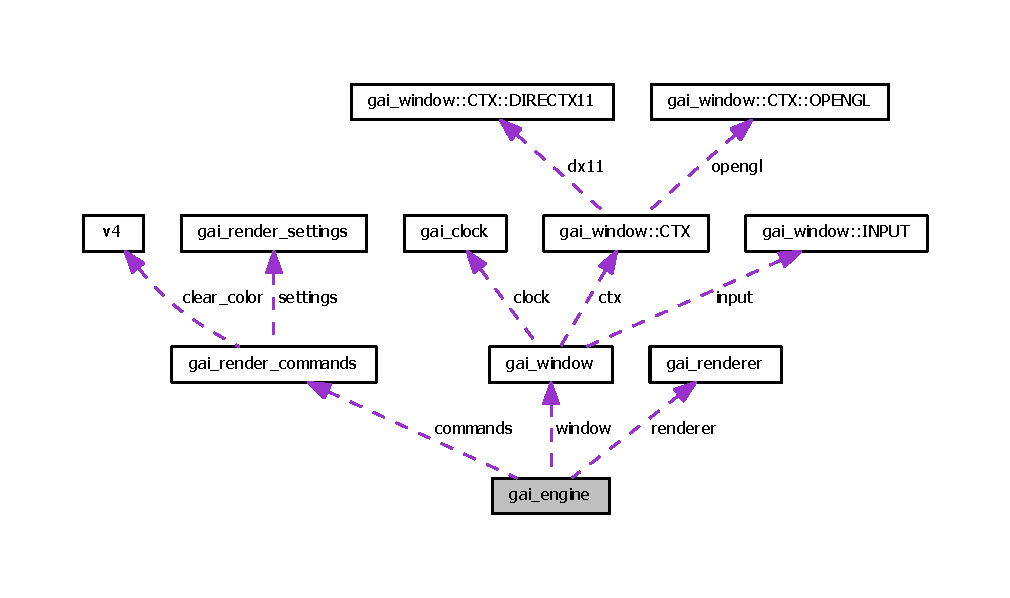
\includegraphics[width=350pt]{structgai__engine__coll__graph}
\end{center}
\end{figure}
\subsection*{Public Attributes}
\begin{DoxyCompactItemize}
\item 
\mbox{\Hypertarget{structgai__engine_a7460be72bda39ea674c38d1e45eed5ac}\label{structgai__engine_a7460be72bda39ea674c38d1e45eed5ac}} 
\hyperlink{structgai__window}{gai\+\_\+window} {\bfseries window}
\item 
\mbox{\Hypertarget{structgai__engine_a62a2f0b98a5fad5292229b9e1df42430}\label{structgai__engine_a62a2f0b98a5fad5292229b9e1df42430}} 
\hyperlink{structgai__render__commands}{gai\+\_\+render\+\_\+commands} {\bfseries commands}
\item 
\mbox{\Hypertarget{structgai__engine_adbeafcc6f92b0c4872671ceab7c78eb4}\label{structgai__engine_adbeafcc6f92b0c4872671ceab7c78eb4}} 
\hyperlink{uniongai__renderer}{gai\+\_\+renderer} {\bfseries renderer}
\end{DoxyCompactItemize}


\subsection{Member Data Documentation}
\mbox{\Hypertarget{structgai__engine_a62a2f0b98a5fad5292229b9e1df42430}\label{structgai__engine_a62a2f0b98a5fad5292229b9e1df42430}} 
\index{gai\+\_\+engine@{gai\+\_\+engine}!commands@{commands}}
\index{commands@{commands}!gai\+\_\+engine@{gai\+\_\+engine}}
\subsubsection{\texorpdfstring{commands}{commands}}
{\footnotesize\ttfamily \hyperlink{structgai__render__commands}{gai\+\_\+render\+\_\+commands} gai\+\_\+engine\+::commands}

\mbox{\Hypertarget{structgai__engine_adbeafcc6f92b0c4872671ceab7c78eb4}\label{structgai__engine_adbeafcc6f92b0c4872671ceab7c78eb4}} 
\index{gai\+\_\+engine@{gai\+\_\+engine}!renderer@{renderer}}
\index{renderer@{renderer}!gai\+\_\+engine@{gai\+\_\+engine}}
\subsubsection{\texorpdfstring{renderer}{renderer}}
{\footnotesize\ttfamily \hyperlink{uniongai__renderer}{gai\+\_\+renderer} gai\+\_\+engine\+::renderer}

\mbox{\Hypertarget{structgai__engine_a7460be72bda39ea674c38d1e45eed5ac}\label{structgai__engine_a7460be72bda39ea674c38d1e45eed5ac}} 
\index{gai\+\_\+engine@{gai\+\_\+engine}!window@{window}}
\index{window@{window}!gai\+\_\+engine@{gai\+\_\+engine}}
\subsubsection{\texorpdfstring{window}{window}}
{\footnotesize\ttfamily \hyperlink{structgai__window}{gai\+\_\+window} gai\+\_\+engine\+::window}



The documentation for this struct was generated from the following file\+:\begin{DoxyCompactItemize}
\item 
gai\+\_\+engine.\+h\end{DoxyCompactItemize}

\hypertarget{structgai__engine__platform__api}{}\section{gai\+\_\+engine\+\_\+platform\+\_\+api Struct Reference}
\label{structgai__engine__platform__api}\index{gai\+\_\+engine\+\_\+platform\+\_\+api@{gai\+\_\+engine\+\_\+platform\+\_\+api}}
\subsection*{Public Attributes}
\begin{DoxyCompactItemize}
\item 
\mbox{\Hypertarget{structgai__engine__platform__api_a55b635f160edefc0148f1e5d49ff080f}\label{structgai__engine__platform__api_a55b635f160edefc0148f1e5d49ff080f}} 
impl\+\_\+platform\+\_\+alloc $\ast$ {\bfseries alloc}
\item 
\mbox{\Hypertarget{structgai__engine__platform__api_a464dadc9755ae2ecba58bc4aca1b6e65}\label{structgai__engine__platform__api_a464dadc9755ae2ecba58bc4aca1b6e65}} 
impl\+\_\+platform\+\_\+free $\ast$ {\bfseries free}
\item 
\mbox{\Hypertarget{structgai__engine__platform__api_a9ee2b129221d6c1472b413a7349d2e43}\label{structgai__engine__platform__api_a9ee2b129221d6c1472b413a7349d2e43}} 
impl\+\_\+platform\+\_\+read\+\_\+file\+\_\+content $\ast$ {\bfseries read\+\_\+file\+\_\+content}
\item 
\mbox{\Hypertarget{structgai__engine__platform__api_a2607e3908f036c0aa4af0edb55315503}\label{structgai__engine__platform__api_a2607e3908f036c0aa4af0edb55315503}} 
impl\+\_\+platform\+\_\+free\+\_\+file\+\_\+memory $\ast$ {\bfseries free\+\_\+file\+\_\+memory}
\end{DoxyCompactItemize}


\subsection{Member Data Documentation}
\mbox{\Hypertarget{structgai__engine__platform__api_a55b635f160edefc0148f1e5d49ff080f}\label{structgai__engine__platform__api_a55b635f160edefc0148f1e5d49ff080f}} 
\index{gai\+\_\+engine\+\_\+platform\+\_\+api@{gai\+\_\+engine\+\_\+platform\+\_\+api}!alloc@{alloc}}
\index{alloc@{alloc}!gai\+\_\+engine\+\_\+platform\+\_\+api@{gai\+\_\+engine\+\_\+platform\+\_\+api}}
\subsubsection{\texorpdfstring{alloc}{alloc}}
{\footnotesize\ttfamily impl\+\_\+platform\+\_\+alloc$\ast$ gai\+\_\+engine\+\_\+platform\+\_\+api\+::alloc}

\mbox{\Hypertarget{structgai__engine__platform__api_a464dadc9755ae2ecba58bc4aca1b6e65}\label{structgai__engine__platform__api_a464dadc9755ae2ecba58bc4aca1b6e65}} 
\index{gai\+\_\+engine\+\_\+platform\+\_\+api@{gai\+\_\+engine\+\_\+platform\+\_\+api}!free@{free}}
\index{free@{free}!gai\+\_\+engine\+\_\+platform\+\_\+api@{gai\+\_\+engine\+\_\+platform\+\_\+api}}
\subsubsection{\texorpdfstring{free}{free}}
{\footnotesize\ttfamily impl\+\_\+platform\+\_\+free$\ast$ gai\+\_\+engine\+\_\+platform\+\_\+api\+::free}

\mbox{\Hypertarget{structgai__engine__platform__api_a2607e3908f036c0aa4af0edb55315503}\label{structgai__engine__platform__api_a2607e3908f036c0aa4af0edb55315503}} 
\index{gai\+\_\+engine\+\_\+platform\+\_\+api@{gai\+\_\+engine\+\_\+platform\+\_\+api}!free\+\_\+file\+\_\+memory@{free\+\_\+file\+\_\+memory}}
\index{free\+\_\+file\+\_\+memory@{free\+\_\+file\+\_\+memory}!gai\+\_\+engine\+\_\+platform\+\_\+api@{gai\+\_\+engine\+\_\+platform\+\_\+api}}
\subsubsection{\texorpdfstring{free\+\_\+file\+\_\+memory}{free\_file\_memory}}
{\footnotesize\ttfamily impl\+\_\+platform\+\_\+free\+\_\+file\+\_\+memory$\ast$ gai\+\_\+engine\+\_\+platform\+\_\+api\+::free\+\_\+file\+\_\+memory}

\mbox{\Hypertarget{structgai__engine__platform__api_a9ee2b129221d6c1472b413a7349d2e43}\label{structgai__engine__platform__api_a9ee2b129221d6c1472b413a7349d2e43}} 
\index{gai\+\_\+engine\+\_\+platform\+\_\+api@{gai\+\_\+engine\+\_\+platform\+\_\+api}!read\+\_\+file\+\_\+content@{read\+\_\+file\+\_\+content}}
\index{read\+\_\+file\+\_\+content@{read\+\_\+file\+\_\+content}!gai\+\_\+engine\+\_\+platform\+\_\+api@{gai\+\_\+engine\+\_\+platform\+\_\+api}}
\subsubsection{\texorpdfstring{read\+\_\+file\+\_\+content}{read\_file\_content}}
{\footnotesize\ttfamily impl\+\_\+platform\+\_\+read\+\_\+file\+\_\+content$\ast$ gai\+\_\+engine\+\_\+platform\+\_\+api\+::read\+\_\+file\+\_\+content}



The documentation for this struct was generated from the following file\+:\begin{DoxyCompactItemize}
\item 
gai\+\_\+engine.\+h\end{DoxyCompactItemize}

\hypertarget{structgai__engine__setup}{}\section{gai\+\_\+engine\+\_\+setup Struct Reference}
\label{structgai__engine__setup}\index{gai\+\_\+engine\+\_\+setup@{gai\+\_\+engine\+\_\+setup}}
\subsection*{Public Attributes}
\begin{DoxyCompactItemize}
\item 
\mbox{\Hypertarget{structgai__engine__setup_a6f946b7d3c11abef7d0f34b339685ca0}\label{structgai__engine__setup_a6f946b7d3c11abef7d0f34b339685ca0}} 
u32 {\bfseries render\+\_\+buffer\+\_\+size\+\_\+mb}
\item 
\mbox{\Hypertarget{structgai__engine__setup_a6511a76398600b953d5fe6de5041ed7b}\label{structgai__engine__setup_a6511a76398600b953d5fe6de5041ed7b}} 
i32 {\bfseries swap\+\_\+interval}
\item 
\mbox{\Hypertarget{structgai__engine__setup_a1051e0a0e262464dec76fe44732bbef3}\label{structgai__engine__setup_a1051e0a0e262464dec76fe44732bbef3}} 
gai\+\_\+renderer\+\_\+type {\bfseries renderer\+\_\+type}
\item 
\mbox{\Hypertarget{structgai__engine__setup_ac3788affec1830e3b9b0c323c1373ae4}\label{structgai__engine__setup_ac3788affec1830e3b9b0c323c1373ae4}} 
\begin{tabbing}
xx\=xx\=xx\=xx\=xx\=xx\=xx\=xx\=xx\=\kill
union \{\\
\mbox{\Hypertarget{structgai__engine__setup_ab9fa247fb71f3648eb64cf12746a041d}\label{structgai__engine__setup_ab9fa247fb71f3648eb64cf12746a041d}} 
\>struct \{\\
\mbox{\Hypertarget{structgai__engine__setup_1_1_0D20_1_1_0D22_adee746fb694c45f01126ea2706b9bbc5}\label{structgai__engine__setup_1_1_0D20_1_1_0D22_adee746fb694c45f01126ea2706b9bbc5}} 
i32 {\bfseries major}\\
\mbox{\Hypertarget{structgai__engine__setup_1_1_0D20_1_1_0D22_aaab4b80635264db989253dee98ea5b2e}\label{structgai__engine__setup_1_1_0D20_1_1_0D22_aaab4b80635264db989253dee98ea5b2e}} 
i32 {\bfseries minor}\\
\mbox{\Hypertarget{structgai__engine__setup_1_1_0D20_1_1_0D22_aa3acd90eebdceffcf9a2dac135a87ac5}\label{structgai__engine__setup_1_1_0D20_1_1_0D22_aa3acd90eebdceffcf9a2dac135a87ac5}} 
i32 {\bfseries core}\\
\mbox{\Hypertarget{structgai__engine__setup_1_1_0D20_1_1_0D22_abc2cf2c6535db8b38e544a2e00779aa5}\label{structgai__engine__setup_1_1_0D20_1_1_0D22_abc2cf2c6535db8b38e544a2e00779aa5}} 
i32 {\bfseries debug}\\
\>\} {\bfseries opengl}\\
\}; \\

\end{tabbing}\end{DoxyCompactItemize}


\subsection{Member Data Documentation}
\mbox{\Hypertarget{structgai__engine__setup_ac3788affec1830e3b9b0c323c1373ae4}\label{structgai__engine__setup_ac3788affec1830e3b9b0c323c1373ae4}} 
\subsubsection{\texorpdfstring{"@21}{@21}}
{\footnotesize\ttfamily union \{ ... \} }

\mbox{\Hypertarget{structgai__engine__setup_a6f946b7d3c11abef7d0f34b339685ca0}\label{structgai__engine__setup_a6f946b7d3c11abef7d0f34b339685ca0}} 
\index{gai\+\_\+engine\+\_\+setup@{gai\+\_\+engine\+\_\+setup}!render\+\_\+buffer\+\_\+size\+\_\+mb@{render\+\_\+buffer\+\_\+size\+\_\+mb}}
\index{render\+\_\+buffer\+\_\+size\+\_\+mb@{render\+\_\+buffer\+\_\+size\+\_\+mb}!gai\+\_\+engine\+\_\+setup@{gai\+\_\+engine\+\_\+setup}}
\subsubsection{\texorpdfstring{render\+\_\+buffer\+\_\+size\+\_\+mb}{render\_buffer\_size\_mb}}
{\footnotesize\ttfamily u32 gai\+\_\+engine\+\_\+setup\+::render\+\_\+buffer\+\_\+size\+\_\+mb}

\mbox{\Hypertarget{structgai__engine__setup_a1051e0a0e262464dec76fe44732bbef3}\label{structgai__engine__setup_a1051e0a0e262464dec76fe44732bbef3}} 
\index{gai\+\_\+engine\+\_\+setup@{gai\+\_\+engine\+\_\+setup}!renderer\+\_\+type@{renderer\+\_\+type}}
\index{renderer\+\_\+type@{renderer\+\_\+type}!gai\+\_\+engine\+\_\+setup@{gai\+\_\+engine\+\_\+setup}}
\subsubsection{\texorpdfstring{renderer\+\_\+type}{renderer\_type}}
{\footnotesize\ttfamily gai\+\_\+renderer\+\_\+type gai\+\_\+engine\+\_\+setup\+::renderer\+\_\+type}

\mbox{\Hypertarget{structgai__engine__setup_a6511a76398600b953d5fe6de5041ed7b}\label{structgai__engine__setup_a6511a76398600b953d5fe6de5041ed7b}} 
\index{gai\+\_\+engine\+\_\+setup@{gai\+\_\+engine\+\_\+setup}!swap\+\_\+interval@{swap\+\_\+interval}}
\index{swap\+\_\+interval@{swap\+\_\+interval}!gai\+\_\+engine\+\_\+setup@{gai\+\_\+engine\+\_\+setup}}
\subsubsection{\texorpdfstring{swap\+\_\+interval}{swap\_interval}}
{\footnotesize\ttfamily i32 gai\+\_\+engine\+\_\+setup\+::swap\+\_\+interval}



The documentation for this struct was generated from the following file\+:\begin{DoxyCompactItemize}
\item 
gai\+\_\+engine.\+h\end{DoxyCompactItemize}

\hypertarget{uniongai__engine__setup_8____unnamed____}{}\section{gai\+\_\+engine\+\_\+setup.\+\_\+\+\_\+unnamed\+\_\+\+\_\+ Union Reference}
\label{uniongai__engine__setup_8____unnamed____}\index{gai\+\_\+engine\+\_\+setup.\+\_\+\+\_\+unnamed\+\_\+\+\_\+@{gai\+\_\+engine\+\_\+setup.\+\_\+\+\_\+unnamed\+\_\+\+\_\+}}
\subsection*{Public Attributes}
\begin{DoxyCompactItemize}
\item 
\mbox{\Hypertarget{uniongai__engine__setup_8____unnamed_____a6785e6b975db5d7cf223101ef1bc2f6f}\label{uniongai__engine__setup_8____unnamed_____a6785e6b975db5d7cf223101ef1bc2f6f}} 
\begin{tabbing}
xx\=xx\=xx\=xx\=xx\=xx\=xx\=xx\=xx\=\kill
struct \{\\
\mbox{\Hypertarget{structgai__engine__setup_1_1_0D20_1_1_0D22_adee746fb694c45f01126ea2706b9bbc5}\label{structgai__engine__setup_1_1_0D20_1_1_0D22_adee746fb694c45f01126ea2706b9bbc5}} 
i32 {\bfseries major}\\
\mbox{\Hypertarget{structgai__engine__setup_1_1_0D20_1_1_0D22_aaab4b80635264db989253dee98ea5b2e}\label{structgai__engine__setup_1_1_0D20_1_1_0D22_aaab4b80635264db989253dee98ea5b2e}} 
i32 {\bfseries minor}\\
\mbox{\Hypertarget{structgai__engine__setup_1_1_0D20_1_1_0D22_aa3acd90eebdceffcf9a2dac135a87ac5}\label{structgai__engine__setup_1_1_0D20_1_1_0D22_aa3acd90eebdceffcf9a2dac135a87ac5}} 
i32 {\bfseries core}\\
\mbox{\Hypertarget{structgai__engine__setup_1_1_0D20_1_1_0D22_abc2cf2c6535db8b38e544a2e00779aa5}\label{structgai__engine__setup_1_1_0D20_1_1_0D22_abc2cf2c6535db8b38e544a2e00779aa5}} 
i32 {\bfseries debug}\\
\} {\bfseries opengl}\\

\end{tabbing}\end{DoxyCompactItemize}


\subsection{Member Data Documentation}
\mbox{\Hypertarget{uniongai__engine__setup_8____unnamed_____a6785e6b975db5d7cf223101ef1bc2f6f}\label{uniongai__engine__setup_8____unnamed_____a6785e6b975db5d7cf223101ef1bc2f6f}} 
\index{gai\+\_\+engine\+\_\+setup.\+\_\+\+\_\+unnamed\+\_\+\+\_\+@{gai\+\_\+engine\+\_\+setup.\+\_\+\+\_\+unnamed\+\_\+\+\_\+}!opengl@{opengl}}
\index{opengl@{opengl}!gai\+\_\+engine\+\_\+setup.\+\_\+\+\_\+unnamed\+\_\+\+\_\+@{gai\+\_\+engine\+\_\+setup.\+\_\+\+\_\+unnamed\+\_\+\+\_\+}}
\subsubsection{\texorpdfstring{opengl}{opengl}}
{\footnotesize\ttfamily }



The documentation for this union was generated from the following files\+:
\hypertarget{structgai__engine__setup_8____unnamed_____8opengl}{}\section{gai\+\_\+engine\+\_\+setup.\+\_\+\+\_\+unnamed\+\_\+\+\_\+.\+opengl Struct Reference}
\label{structgai__engine__setup_8____unnamed_____8opengl}\index{gai\+\_\+engine\+\_\+setup.\+\_\+\+\_\+unnamed\+\_\+\+\_\+.\+opengl@{gai\+\_\+engine\+\_\+setup.\+\_\+\+\_\+unnamed\+\_\+\+\_\+.\+opengl}}
\subsection*{Public Attributes}
\begin{DoxyCompactItemize}
\item 
\mbox{\Hypertarget{structgai__engine__setup_8____unnamed_____8opengl_af1425da40a9f2d21ab702a1c7feae026}\label{structgai__engine__setup_8____unnamed_____8opengl_af1425da40a9f2d21ab702a1c7feae026}} 
i32 {\bfseries major}
\item 
\mbox{\Hypertarget{structgai__engine__setup_8____unnamed_____8opengl_aab846c0e3717a3e7d14af45cab70b44a}\label{structgai__engine__setup_8____unnamed_____8opengl_aab846c0e3717a3e7d14af45cab70b44a}} 
i32 {\bfseries minor}
\item 
\mbox{\Hypertarget{structgai__engine__setup_8____unnamed_____8opengl_aa74ad8dfacd4f985eb3977517615ce25}\label{structgai__engine__setup_8____unnamed_____8opengl_aa74ad8dfacd4f985eb3977517615ce25}} 
i32 {\bfseries core}
\item 
\mbox{\Hypertarget{structgai__engine__setup_8____unnamed_____8opengl_aad42f6697b035b7580e4fef93be20b4d}\label{structgai__engine__setup_8____unnamed_____8opengl_aad42f6697b035b7580e4fef93be20b4d}} 
i32 {\bfseries debug}
\end{DoxyCompactItemize}


\subsection{Member Data Documentation}
\mbox{\Hypertarget{structgai__engine__setup_8____unnamed_____8opengl_aa74ad8dfacd4f985eb3977517615ce25}\label{structgai__engine__setup_8____unnamed_____8opengl_aa74ad8dfacd4f985eb3977517615ce25}} 
\index{gai\+\_\+engine\+\_\+setup.\+\_\+\+\_\+unnamed\+\_\+\+\_\+.\+opengl@{gai\+\_\+engine\+\_\+setup.\+\_\+\+\_\+unnamed\+\_\+\+\_\+.\+opengl}!core@{core}}
\index{core@{core}!gai\+\_\+engine\+\_\+setup.\+\_\+\+\_\+unnamed\+\_\+\+\_\+.\+opengl@{gai\+\_\+engine\+\_\+setup.\+\_\+\+\_\+unnamed\+\_\+\+\_\+.\+opengl}}
\subsubsection{\texorpdfstring{core}{core}}
{\footnotesize\ttfamily }

\mbox{\Hypertarget{structgai__engine__setup_8____unnamed_____8opengl_aad42f6697b035b7580e4fef93be20b4d}\label{structgai__engine__setup_8____unnamed_____8opengl_aad42f6697b035b7580e4fef93be20b4d}} 
\index{gai\+\_\+engine\+\_\+setup.\+\_\+\+\_\+unnamed\+\_\+\+\_\+.\+opengl@{gai\+\_\+engine\+\_\+setup.\+\_\+\+\_\+unnamed\+\_\+\+\_\+.\+opengl}!debug@{debug}}
\index{debug@{debug}!gai\+\_\+engine\+\_\+setup.\+\_\+\+\_\+unnamed\+\_\+\+\_\+.\+opengl@{gai\+\_\+engine\+\_\+setup.\+\_\+\+\_\+unnamed\+\_\+\+\_\+.\+opengl}}
\subsubsection{\texorpdfstring{debug}{debug}}
{\footnotesize\ttfamily }

\mbox{\Hypertarget{structgai__engine__setup_8____unnamed_____8opengl_af1425da40a9f2d21ab702a1c7feae026}\label{structgai__engine__setup_8____unnamed_____8opengl_af1425da40a9f2d21ab702a1c7feae026}} 
\index{gai\+\_\+engine\+\_\+setup.\+\_\+\+\_\+unnamed\+\_\+\+\_\+.\+opengl@{gai\+\_\+engine\+\_\+setup.\+\_\+\+\_\+unnamed\+\_\+\+\_\+.\+opengl}!major@{major}}
\index{major@{major}!gai\+\_\+engine\+\_\+setup.\+\_\+\+\_\+unnamed\+\_\+\+\_\+.\+opengl@{gai\+\_\+engine\+\_\+setup.\+\_\+\+\_\+unnamed\+\_\+\+\_\+.\+opengl}}
\subsubsection{\texorpdfstring{major}{major}}
{\footnotesize\ttfamily }

\mbox{\Hypertarget{structgai__engine__setup_8____unnamed_____8opengl_aab846c0e3717a3e7d14af45cab70b44a}\label{structgai__engine__setup_8____unnamed_____8opengl_aab846c0e3717a3e7d14af45cab70b44a}} 
\index{gai\+\_\+engine\+\_\+setup.\+\_\+\+\_\+unnamed\+\_\+\+\_\+.\+opengl@{gai\+\_\+engine\+\_\+setup.\+\_\+\+\_\+unnamed\+\_\+\+\_\+.\+opengl}!minor@{minor}}
\index{minor@{minor}!gai\+\_\+engine\+\_\+setup.\+\_\+\+\_\+unnamed\+\_\+\+\_\+.\+opengl@{gai\+\_\+engine\+\_\+setup.\+\_\+\+\_\+unnamed\+\_\+\+\_\+.\+opengl}}
\subsubsection{\texorpdfstring{minor}{minor}}
{\footnotesize\ttfamily }



The documentation for this struct was generated from the following files\+:
\hypertarget{structgai__loaded__file}{}\section{gai\+\_\+loaded\+\_\+file Struct Reference}
\label{structgai__loaded__file}\index{gai\+\_\+loaded\+\_\+file@{gai\+\_\+loaded\+\_\+file}}
\subsection*{Public Attributes}
\begin{DoxyCompactItemize}
\item 
\mbox{\Hypertarget{structgai__loaded__file_a16e4244cb0fba12420c0499828c0dfec}\label{structgai__loaded__file_a16e4244cb0fba12420c0499828c0dfec}} 
unsigned int {\bfseries size}
\item 
\mbox{\Hypertarget{structgai__loaded__file_a701c480c708004b79c5028835816554c}\label{structgai__loaded__file_a701c480c708004b79c5028835816554c}} 
void $\ast$ {\bfseries data}
\end{DoxyCompactItemize}


\subsection{Member Data Documentation}
\mbox{\Hypertarget{structgai__loaded__file_a701c480c708004b79c5028835816554c}\label{structgai__loaded__file_a701c480c708004b79c5028835816554c}} 
\index{gai\+\_\+loaded\+\_\+file@{gai\+\_\+loaded\+\_\+file}!data@{data}}
\index{data@{data}!gai\+\_\+loaded\+\_\+file@{gai\+\_\+loaded\+\_\+file}}
\subsubsection{\texorpdfstring{data}{data}}
{\footnotesize\ttfamily void$\ast$ gai\+\_\+loaded\+\_\+file\+::data}

\mbox{\Hypertarget{structgai__loaded__file_a16e4244cb0fba12420c0499828c0dfec}\label{structgai__loaded__file_a16e4244cb0fba12420c0499828c0dfec}} 
\index{gai\+\_\+loaded\+\_\+file@{gai\+\_\+loaded\+\_\+file}!size@{size}}
\index{size@{size}!gai\+\_\+loaded\+\_\+file@{gai\+\_\+loaded\+\_\+file}}
\subsubsection{\texorpdfstring{size}{size}}
{\footnotesize\ttfamily unsigned int gai\+\_\+loaded\+\_\+file\+::size}



The documentation for this struct was generated from the following file\+:\begin{DoxyCompactItemize}
\item 
gai\+\_\+engine.\+h\end{DoxyCompactItemize}

\hypertarget{structgai__render__commands}{}\section{gai\+\_\+render\+\_\+commands Struct Reference}
\label{structgai__render__commands}\index{gai\+\_\+render\+\_\+commands@{gai\+\_\+render\+\_\+commands}}


Collaboration diagram for gai\+\_\+render\+\_\+commands\+:\nopagebreak
\begin{figure}[H]
\begin{center}
\leavevmode
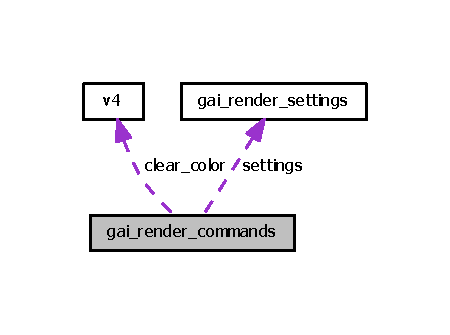
\includegraphics[width=216pt]{structgai__render__commands__coll__graph}
\end{center}
\end{figure}
\subsection*{Public Member Functions}
\begin{DoxyCompactItemize}
\item 
\mbox{\Hypertarget{structgai__render__commands_a3e2bcf7118cbc84c5615486ac1f8b221}\label{structgai__render__commands_a3e2bcf7118cbc84c5615486ac1f8b221}} 
{\bfseries gai\+\_\+growable} (\hyperlink{structtextured__vertex}{textured\+\_\+vertex}) vertices
\end{DoxyCompactItemize}
\subsection*{Public Attributes}
\begin{DoxyCompactItemize}
\item 
\mbox{\Hypertarget{structgai__render__commands_abdcadaebc26e8673763975e406c56b0c}\label{structgai__render__commands_abdcadaebc26e8673763975e406c56b0c}} 
\hyperlink{structgai__render__settings}{gai\+\_\+render\+\_\+settings} {\bfseries settings}
\item 
\mbox{\Hypertarget{structgai__render__commands_a05da5b761fee8979f03aea81fc18e7e2}\label{structgai__render__commands_a05da5b761fee8979f03aea81fc18e7e2}} 
u32 {\bfseries pushbuffer\+\_\+max}
\item 
\mbox{\Hypertarget{structgai__render__commands_a8cdb202f3a17cdc5ff2cc5fdfbbb9182}\label{structgai__render__commands_a8cdb202f3a17cdc5ff2cc5fdfbbb9182}} 
u8 $\ast$ {\bfseries pushbuffer\+\_\+base}
\item 
\mbox{\Hypertarget{structgai__render__commands_a6b900436d146ec352a75d875c8908a91}\label{structgai__render__commands_a6b900436d146ec352a75d875c8908a91}} 
u8 $\ast$ {\bfseries pushbuffer\+\_\+at}
\item 
\mbox{\Hypertarget{structgai__render__commands_a3f036f20e85d6497ab888f0dd3772056}\label{structgai__render__commands_a3f036f20e85d6497ab888f0dd3772056}} 
\hyperlink{unionv4}{v4} {\bfseries clear\+\_\+color}
\end{DoxyCompactItemize}


The documentation for this struct was generated from the following file\+:\begin{DoxyCompactItemize}
\item 
gai\+\_\+engine.\+h\end{DoxyCompactItemize}

\hypertarget{structgai__render__settings}{}\section{gai\+\_\+render\+\_\+settings Struct Reference}
\label{structgai__render__settings}\index{gai\+\_\+render\+\_\+settings@{gai\+\_\+render\+\_\+settings}}
\subsection*{Public Attributes}
\begin{DoxyCompactItemize}
\item 
\mbox{\Hypertarget{structgai__render__settings_a94158f4aeba7ee4619d7ef64fe882b79}\label{structgai__render__settings_a94158f4aeba7ee4619d7ef64fe882b79}} 
u32 {\bfseries width}
\item 
\mbox{\Hypertarget{structgai__render__settings_a646f141e340397c5a7d51f2c448f8bc6}\label{structgai__render__settings_a646f141e340397c5a7d51f2c448f8bc6}} 
u32 {\bfseries height}
\end{DoxyCompactItemize}


\subsection{Member Data Documentation}
\mbox{\Hypertarget{structgai__render__settings_a646f141e340397c5a7d51f2c448f8bc6}\label{structgai__render__settings_a646f141e340397c5a7d51f2c448f8bc6}} 
\index{gai\+\_\+render\+\_\+settings@{gai\+\_\+render\+\_\+settings}!height@{height}}
\index{height@{height}!gai\+\_\+render\+\_\+settings@{gai\+\_\+render\+\_\+settings}}
\subsubsection{\texorpdfstring{height}{height}}
{\footnotesize\ttfamily u32 gai\+\_\+render\+\_\+settings\+::height}

\mbox{\Hypertarget{structgai__render__settings_a94158f4aeba7ee4619d7ef64fe882b79}\label{structgai__render__settings_a94158f4aeba7ee4619d7ef64fe882b79}} 
\index{gai\+\_\+render\+\_\+settings@{gai\+\_\+render\+\_\+settings}!width@{width}}
\index{width@{width}!gai\+\_\+render\+\_\+settings@{gai\+\_\+render\+\_\+settings}}
\subsubsection{\texorpdfstring{width}{width}}
{\footnotesize\ttfamily u32 gai\+\_\+render\+\_\+settings\+::width}



The documentation for this struct was generated from the following file\+:\begin{DoxyCompactItemize}
\item 
gai\+\_\+engine.\+h\end{DoxyCompactItemize}

\hypertarget{uniongai__renderer}{}\section{gai\+\_\+renderer Union Reference}
\label{uniongai__renderer}\index{gai\+\_\+renderer@{gai\+\_\+renderer}}
\subsection*{Public Attributes}
\begin{DoxyCompactItemize}
\item 
\mbox{\Hypertarget{uniongai__renderer_ab39127ce67280acdc56451722184f2f0}\label{uniongai__renderer_ab39127ce67280acdc56451722184f2f0}} 
gai\+\_\+renderer\+\_\+opengl {\bfseries opengl}
\end{DoxyCompactItemize}


\subsection{Member Data Documentation}
\mbox{\Hypertarget{uniongai__renderer_ab39127ce67280acdc56451722184f2f0}\label{uniongai__renderer_ab39127ce67280acdc56451722184f2f0}} 
\index{gai\+\_\+renderer@{gai\+\_\+renderer}!opengl@{opengl}}
\index{opengl@{opengl}!gai\+\_\+renderer@{gai\+\_\+renderer}}
\subsubsection{\texorpdfstring{opengl}{opengl}}
{\footnotesize\ttfamily gai\+\_\+renderer\+\_\+opengl gai\+\_\+renderer\+::opengl}



The documentation for this union was generated from the following file\+:\begin{DoxyCompactItemize}
\item 
gai\+\_\+engine.\+h\end{DoxyCompactItemize}

\hypertarget{structgai__window}{}\section{gai\+\_\+window Struct Reference}
\label{structgai__window}\index{gai\+\_\+window@{gai\+\_\+window}}


Collaboration diagram for gai\+\_\+window\+:\nopagebreak
\begin{figure}[H]
\begin{center}
\leavevmode
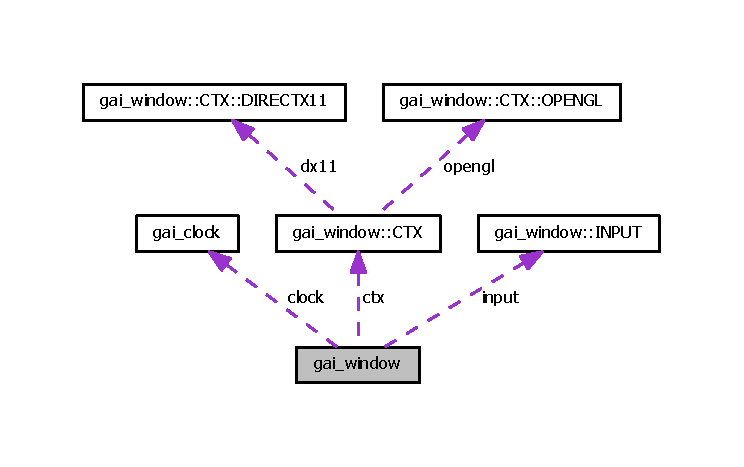
\includegraphics[width=350pt]{structgai__window__coll__graph}
\end{center}
\end{figure}
\subsection*{Classes}
\begin{DoxyCompactItemize}
\item 
union \hyperlink{structgai__window_uniongai__window_1_1_c_t_x}{C\+TX}
\item 
struct \hyperlink{structgai__window_structgai__window_1_1_i_n_p_u_t}{I\+N\+P\+UT}
\end{DoxyCompactItemize}
\subsection*{Public Member Functions}
\begin{DoxyCompactItemize}
\item 
\mbox{\Hypertarget{structgai__window_a5ef904435ae2d6ac768e856ac809393d}\label{structgai__window_a5ef904435ae2d6ac768e856ac809393d}} 
{\bfseries gai\+\_\+growable} (\hyperlink{gai_8h_structgai__window__callback}{gai\+\_\+window\+\_\+callback}) callbacks
\end{DoxyCompactItemize}
\subsection*{Public Attributes}
\begin{DoxyCompactItemize}
\item 
\mbox{\Hypertarget{structgai__window_a9ccc16f8ea46bcf16f97bb7ad6718c5a}\label{structgai__window_a9ccc16f8ea46bcf16f97bb7ad6718c5a}} 
void $\ast$ {\bfseries handle}
\item 
\mbox{\Hypertarget{structgai__window_a8f79768a9175a0700317a60c64a9f1d6}\label{structgai__window_a8f79768a9175a0700317a60c64a9f1d6}} 
W\+I\+N\+D\+O\+W\+P\+L\+A\+C\+E\+M\+E\+NT {\bfseries placement\+\_\+win32}
\item 
\mbox{\Hypertarget{structgai__window_a23db179b60e7dfc4d8dfc7792dfb5501}\label{structgai__window_a23db179b60e7dfc4d8dfc7792dfb5501}} 
i32 {\bfseries x}
\item 
\mbox{\Hypertarget{structgai__window_a280b39609526727ad16abf166a6054f1}\label{structgai__window_a280b39609526727ad16abf166a6054f1}} 
i32 {\bfseries y}
\item 
\mbox{\Hypertarget{structgai__window_adb9910632580296999c3785eba2ebc48}\label{structgai__window_adb9910632580296999c3785eba2ebc48}} 
i32 {\bfseries w}
\item 
\mbox{\Hypertarget{structgai__window_a7ae67a6eb8a37a93a56eb2f882531bfa}\label{structgai__window_a7ae67a6eb8a37a93a56eb2f882531bfa}} 
i32 {\bfseries h}
\item 
\mbox{\Hypertarget{structgai__window_a7f2295e5b493ee66c97a2e65062db6d1}\label{structgai__window_a7f2295e5b493ee66c97a2e65062db6d1}} 
u32 {\bfseries flags}
\item 
\mbox{\Hypertarget{structgai__window_aea0a3b7e016ff3ec326f8d9e45a9d321}\label{structgai__window_aea0a3b7e016ff3ec326f8d9e45a9d321}} 
r64 {\bfseries dt}
\item 
\mbox{\Hypertarget{structgai__window_a88e46311d090dd0e65c26dfc8bf302e4}\label{structgai__window_a88e46311d090dd0e65c26dfc8bf302e4}} 
u32 {\bfseries was\+\_\+closed}
\item 
\mbox{\Hypertarget{structgai__window_a10780aa6154e42c0ab7ec981d1ccabae}\label{structgai__window_a10780aa6154e42c0ab7ec981d1ccabae}} 
u32 {\bfseries request\+\_\+close}
\item 
\mbox{\Hypertarget{structgai__window_a8e7a2d4309b6eb57601aa7e79072d1dd}\label{structgai__window_a8e7a2d4309b6eb57601aa7e79072d1dd}} 
gai\+\_\+renderer\+\_\+type {\bfseries type}
\item 
\mbox{\Hypertarget{structgai__window_ae0483cf458672fc68c6f000670102b45}\label{structgai__window_ae0483cf458672fc68c6f000670102b45}} 
union \hyperlink{structgai__window_uniongai__window_1_1_c_t_x}{gai\+\_\+window\+::\+C\+TX} {\bfseries ctx}
\item 
\mbox{\Hypertarget{structgai__window_a73a5158ee13d09c11968ff8237542c8b}\label{structgai__window_a73a5158ee13d09c11968ff8237542c8b}} 
struct \hyperlink{structgai__window_structgai__window_1_1_i_n_p_u_t}{gai\+\_\+window\+::\+I\+N\+P\+UT} {\bfseries input}
\item 
\mbox{\Hypertarget{structgai__window_a726b3b659d1af3101f4c1a7228bf3950}\label{structgai__window_a726b3b659d1af3101f4c1a7228bf3950}} 
\hyperlink{gai_8h_structgai__clock}{gai\+\_\+clock} {\bfseries clock}
\end{DoxyCompactItemize}


\subsection{Class Documentation}
\index{gai\+\_\+window\+::\+C\+TX@{gai\+\_\+window\+::\+C\+TX}}\label{uniongai__window_1_1_c_t_x}
\Hypertarget{structgai__window_uniongai__window_1_1_c_t_x}
\subsubsection{union gai\+\_\+window\+:\+:C\+TX}


Collaboration diagram for gai\+\_\+window\+:\+:C\+TX\+:
\nopagebreak
\begin{figure}[H]
\begin{center}
\leavevmode
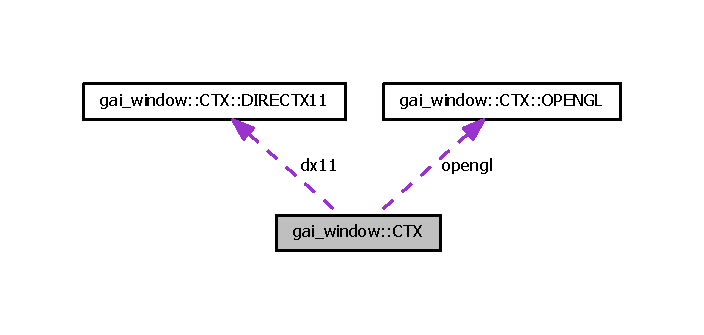
\includegraphics[width=338pt]{uniongai__window_1_1_c_t_x__coll__graph}
\end{center}
\end{figure}
\begin{DoxyFields}{Class Members}
\mbox{\Hypertarget{structgai__window_a2112189a9a1bc9b668a7c75a5527a52d}\label{structgai__window_a2112189a9a1bc9b668a7c75a5527a52d}} 
struct \hyperlink{structgai__window_structgai__window_1_1_c_t_x_1_1_d_i_r_e_c_t_x11}{DIRECTX11}&
dx11&
\\
\hline

\mbox{\Hypertarget{structgai__window_a2b95d5e69bdf2e65fa3bafc4061d0ec7}\label{structgai__window_a2b95d5e69bdf2e65fa3bafc4061d0ec7}} 
struct \hyperlink{structgai__window_structgai__window_1_1_c_t_x_1_1_o_p_e_n_g_l}{OPENGL}&
opengl&
\\
\hline

\end{DoxyFields}
\index{gai\+\_\+window\+::\+I\+N\+P\+UT@{gai\+\_\+window\+::\+I\+N\+P\+UT}}\label{structgai__window_1_1_i_n_p_u_t}
\Hypertarget{structgai__window_structgai__window_1_1_i_n_p_u_t}
\subsubsection{struct gai\+\_\+window\+:\+:I\+N\+P\+UT}
\begin{DoxyFields}{Class Members}
\mbox{\Hypertarget{structgai__window_ad71dabdbe261a269c52bde2c8509dda7}\label{structgai__window_ad71dabdbe261a269c52bde2c8509dda7}} 
gai\_key\_state&
keyboard\_keys\mbox{[}255\mbox{]}&
\\
\hline

\mbox{\Hypertarget{structgai__window_ac74ee49ef25854725042f071982280ae}\label{structgai__window_ac74ee49ef25854725042f071982280ae}} 
gai\_key\_state&
mouse\_buttons\mbox{[}5\mbox{]}&
\\
\hline

\mbox{\Hypertarget{structgai__window_ae768fbdf4db1fd19b9a501b197ca9176}\label{structgai__window_ae768fbdf4db1fd19b9a501b197ca9176}} 
i32&
mouse\_dx&
\\
\hline

\mbox{\Hypertarget{structgai__window_a7a8a489cec34e1df7d704b4338b1bcea}\label{structgai__window_a7a8a489cec34e1df7d704b4338b1bcea}} 
i32&
mouse\_dy&
\\
\hline

\mbox{\Hypertarget{structgai__window_ab4fdfc85ac0563ad1daebfc354e5b6a4}\label{structgai__window_ab4fdfc85ac0563ad1daebfc354e5b6a4}} 
i32&
mouse\_wheel&
\\
\hline

\mbox{\Hypertarget{structgai__window_aada9bddfeb8748fa82a5c3e648695968}\label{structgai__window_aada9bddfeb8748fa82a5c3e648695968}} 
i32&
mouse\_x&
\\
\hline

\mbox{\Hypertarget{structgai__window_a1bf17e49446857bd04deaffb5e666bc5}\label{structgai__window_a1bf17e49446857bd04deaffb5e666bc5}} 
i32&
mouse\_y&
\\
\hline

\end{DoxyFields}


The documentation for this struct was generated from the following file\+:\begin{DoxyCompactItemize}
\item 
\hyperlink{gai_8h}{gai.\+h}\end{DoxyCompactItemize}

\hypertarget{structmat4}{}\section{mat4 Struct Reference}
\label{structmat4}\index{mat4@{mat4}}
\subsection*{Public Attributes}
\begin{DoxyCompactItemize}
\item 
\mbox{\Hypertarget{structmat4_ad61492e85fcebbb837e4d4874030b060}\label{structmat4_ad61492e85fcebbb837e4d4874030b060}} 
r32 {\bfseries T} \mbox{[}16\mbox{]}
\end{DoxyCompactItemize}


\subsection{Member Data Documentation}
\mbox{\Hypertarget{structmat4_ad61492e85fcebbb837e4d4874030b060}\label{structmat4_ad61492e85fcebbb837e4d4874030b060}} 
\index{mat4@{mat4}!T@{T}}
\index{T@{T}!mat4@{mat4}}
\subsubsection{\texorpdfstring{T}{T}}
{\footnotesize\ttfamily r32 mat4\+::T\mbox{[}16\mbox{]}}



The documentation for this struct was generated from the following file\+:\begin{DoxyCompactItemize}
\item 
gai\+\_\+engine.\+h\end{DoxyCompactItemize}

\hypertarget{structtextured__vertex}{}\section{textured\+\_\+vertex Struct Reference}
\label{structtextured__vertex}\index{textured\+\_\+vertex@{textured\+\_\+vertex}}


Collaboration diagram for textured\+\_\+vertex\+:\nopagebreak
\begin{figure}[H]
\begin{center}
\leavevmode
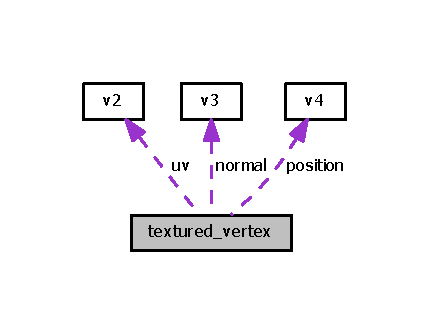
\includegraphics[width=207pt]{structtextured__vertex__coll__graph}
\end{center}
\end{figure}
\subsection*{Public Attributes}
\begin{DoxyCompactItemize}
\item 
\mbox{\Hypertarget{structtextured__vertex_a3c4cd89155276901e97abbea671a5dc3}\label{structtextured__vertex_a3c4cd89155276901e97abbea671a5dc3}} 
\hyperlink{unionv4}{v4} {\bfseries position}
\item 
\mbox{\Hypertarget{structtextured__vertex_a0d7951149447a90843f0474a1f5601ff}\label{structtextured__vertex_a0d7951149447a90843f0474a1f5601ff}} 
\hyperlink{unionv3}{v3} {\bfseries normal}
\item 
\mbox{\Hypertarget{structtextured__vertex_a4301365e41e35082f64868b6ee5193ff}\label{structtextured__vertex_a4301365e41e35082f64868b6ee5193ff}} 
\hyperlink{unionv2}{v2} {\bfseries uv}
\item 
\mbox{\Hypertarget{structtextured__vertex_a73cb353055372f5bd1f42d0dc0802eb2}\label{structtextured__vertex_a73cb353055372f5bd1f42d0dc0802eb2}} 
u32 {\bfseries color}
\end{DoxyCompactItemize}


\subsection{Member Data Documentation}
\mbox{\Hypertarget{structtextured__vertex_a73cb353055372f5bd1f42d0dc0802eb2}\label{structtextured__vertex_a73cb353055372f5bd1f42d0dc0802eb2}} 
\index{textured\+\_\+vertex@{textured\+\_\+vertex}!color@{color}}
\index{color@{color}!textured\+\_\+vertex@{textured\+\_\+vertex}}
\subsubsection{\texorpdfstring{color}{color}}
{\footnotesize\ttfamily u32 textured\+\_\+vertex\+::color}

\mbox{\Hypertarget{structtextured__vertex_a0d7951149447a90843f0474a1f5601ff}\label{structtextured__vertex_a0d7951149447a90843f0474a1f5601ff}} 
\index{textured\+\_\+vertex@{textured\+\_\+vertex}!normal@{normal}}
\index{normal@{normal}!textured\+\_\+vertex@{textured\+\_\+vertex}}
\subsubsection{\texorpdfstring{normal}{normal}}
{\footnotesize\ttfamily \hyperlink{unionv3}{v3} textured\+\_\+vertex\+::normal}

\mbox{\Hypertarget{structtextured__vertex_a3c4cd89155276901e97abbea671a5dc3}\label{structtextured__vertex_a3c4cd89155276901e97abbea671a5dc3}} 
\index{textured\+\_\+vertex@{textured\+\_\+vertex}!position@{position}}
\index{position@{position}!textured\+\_\+vertex@{textured\+\_\+vertex}}
\subsubsection{\texorpdfstring{position}{position}}
{\footnotesize\ttfamily \hyperlink{unionv4}{v4} textured\+\_\+vertex\+::position}

\mbox{\Hypertarget{structtextured__vertex_a4301365e41e35082f64868b6ee5193ff}\label{structtextured__vertex_a4301365e41e35082f64868b6ee5193ff}} 
\index{textured\+\_\+vertex@{textured\+\_\+vertex}!uv@{uv}}
\index{uv@{uv}!textured\+\_\+vertex@{textured\+\_\+vertex}}
\subsubsection{\texorpdfstring{uv}{uv}}
{\footnotesize\ttfamily \hyperlink{unionv2}{v2} textured\+\_\+vertex\+::uv}



The documentation for this struct was generated from the following file\+:\begin{DoxyCompactItemize}
\item 
gai\+\_\+engine.\+h\end{DoxyCompactItemize}

\hypertarget{unionv2}{}\section{v2 Union Reference}
\label{unionv2}\index{v2@{v2}}
\subsection*{Public Attributes}
\begin{DoxyCompactItemize}
\item 
\mbox{\Hypertarget{unionv2_a9973de707fa6afc41c67007de31f7f9d}\label{unionv2_a9973de707fa6afc41c67007de31f7f9d}} 
\begin{tabbing}
xx\=xx\=xx\=xx\=xx\=xx\=xx\=xx\=xx\=\kill
struct \{\\
\mbox{\Hypertarget{unionv2_a208fbec8d559720719fe4b973fbd37b1}\label{unionv2_a208fbec8d559720719fe4b973fbd37b1}} 
r32 {\bfseries x}\\
\mbox{\Hypertarget{unionv2_aa67e08877ab5b9609665dc1d56fa15f4}\label{unionv2_aa67e08877ab5b9609665dc1d56fa15f4}} 
r32 {\bfseries y}\\
\}; \\

\end{tabbing}\item 
\mbox{\Hypertarget{unionv2_abaa590c45431f6a06750196f8775a60f}\label{unionv2_abaa590c45431f6a06750196f8775a60f}} 
\begin{tabbing}
xx\=xx\=xx\=xx\=xx\=xx\=xx\=xx\=xx\=\kill
struct \{\\
\mbox{\Hypertarget{unionv2_aeac8e675916c37ca0cd49e2527668228}\label{unionv2_aeac8e675916c37ca0cd49e2527668228}} 
r32 {\bfseries u}\\
\mbox{\Hypertarget{unionv2_a4f57caa845d978fd3f877f852bd1bdc7}\label{unionv2_a4f57caa845d978fd3f877f852bd1bdc7}} 
r32 {\bfseries v}\\
\}; \\

\end{tabbing}\item 
\mbox{\Hypertarget{unionv2_a64c84ca2180167d5b2966dc34c4396a7}\label{unionv2_a64c84ca2180167d5b2966dc34c4396a7}} 
r32 {\bfseries T} \mbox{[}2\mbox{]}
\end{DoxyCompactItemize}


\subsection{Member Data Documentation}
\mbox{\Hypertarget{unionv2_a9973de707fa6afc41c67007de31f7f9d}\label{unionv2_a9973de707fa6afc41c67007de31f7f9d}} 
\subsubsection{\texorpdfstring{"@5}{@5}}
{\footnotesize\ttfamily struct \{ ... \} }

\mbox{\Hypertarget{unionv2_abaa590c45431f6a06750196f8775a60f}\label{unionv2_abaa590c45431f6a06750196f8775a60f}} 
\subsubsection{\texorpdfstring{"@7}{@7}}
{\footnotesize\ttfamily struct \{ ... \} }

\mbox{\Hypertarget{unionv2_a64c84ca2180167d5b2966dc34c4396a7}\label{unionv2_a64c84ca2180167d5b2966dc34c4396a7}} 
\index{v2@{v2}!T@{T}}
\index{T@{T}!v2@{v2}}
\subsubsection{\texorpdfstring{T}{T}}
{\footnotesize\ttfamily r32 v2\+::T\mbox{[}2\mbox{]}}



The documentation for this union was generated from the following file\+:\begin{DoxyCompactItemize}
\item 
gai\+\_\+engine.\+h\end{DoxyCompactItemize}

\hypertarget{structv2_8____unnamed____}{}\section{v2.\+\_\+\+\_\+unnamed\+\_\+\+\_\+ Struct Reference}
\label{structv2_8____unnamed____}\index{v2.\+\_\+\+\_\+unnamed\+\_\+\+\_\+@{v2.\+\_\+\+\_\+unnamed\+\_\+\+\_\+}}
\subsection*{Public Attributes}
\begin{DoxyCompactItemize}
\item 
\mbox{\Hypertarget{structv2_8____unnamed_____a7b774effe4a349c6dd82ad4f4f21d34c}\label{structv2_8____unnamed_____a7b774effe4a349c6dd82ad4f4f21d34c}} 
r32 {\bfseries u}
\item 
\mbox{\Hypertarget{structv2_8____unnamed_____a9e3669d19b675bd57058fd4664205d2a}\label{structv2_8____unnamed_____a9e3669d19b675bd57058fd4664205d2a}} 
r32 {\bfseries v}
\end{DoxyCompactItemize}


\subsection{Member Data Documentation}
\mbox{\Hypertarget{structv2_8____unnamed_____a7b774effe4a349c6dd82ad4f4f21d34c}\label{structv2_8____unnamed_____a7b774effe4a349c6dd82ad4f4f21d34c}} 
\index{v2.\+\_\+\+\_\+unnamed\+\_\+\+\_\+@{v2.\+\_\+\+\_\+unnamed\+\_\+\+\_\+}!u@{u}}
\index{u@{u}!v2.\+\_\+\+\_\+unnamed\+\_\+\+\_\+@{v2.\+\_\+\+\_\+unnamed\+\_\+\+\_\+}}
\subsubsection{\texorpdfstring{u}{u}}
{\footnotesize\ttfamily }

\mbox{\Hypertarget{structv2_8____unnamed_____a9e3669d19b675bd57058fd4664205d2a}\label{structv2_8____unnamed_____a9e3669d19b675bd57058fd4664205d2a}} 
\index{v2.\+\_\+\+\_\+unnamed\+\_\+\+\_\+@{v2.\+\_\+\+\_\+unnamed\+\_\+\+\_\+}!v@{v}}
\index{v@{v}!v2.\+\_\+\+\_\+unnamed\+\_\+\+\_\+@{v2.\+\_\+\+\_\+unnamed\+\_\+\+\_\+}}
\subsubsection{\texorpdfstring{v}{v}}
{\footnotesize\ttfamily }



The documentation for this struct was generated from the following files\+:
\hypertarget{structv2_8____unnamed____}{}\section{v2.\+\_\+\+\_\+unnamed\+\_\+\+\_\+ Struct Reference}
\label{structv2_8____unnamed____}\index{v2.\+\_\+\+\_\+unnamed\+\_\+\+\_\+@{v2.\+\_\+\+\_\+unnamed\+\_\+\+\_\+}}
\subsection*{Public Attributes}
\begin{DoxyCompactItemize}
\item 
\mbox{\Hypertarget{structv2_8____unnamed_____a7b774effe4a349c6dd82ad4f4f21d34c}\label{structv2_8____unnamed_____a7b774effe4a349c6dd82ad4f4f21d34c}} 
r32 {\bfseries u}
\item 
\mbox{\Hypertarget{structv2_8____unnamed_____a9e3669d19b675bd57058fd4664205d2a}\label{structv2_8____unnamed_____a9e3669d19b675bd57058fd4664205d2a}} 
r32 {\bfseries v}
\end{DoxyCompactItemize}


\subsection{Member Data Documentation}
\mbox{\Hypertarget{structv2_8____unnamed_____a7b774effe4a349c6dd82ad4f4f21d34c}\label{structv2_8____unnamed_____a7b774effe4a349c6dd82ad4f4f21d34c}} 
\index{v2.\+\_\+\+\_\+unnamed\+\_\+\+\_\+@{v2.\+\_\+\+\_\+unnamed\+\_\+\+\_\+}!u@{u}}
\index{u@{u}!v2.\+\_\+\+\_\+unnamed\+\_\+\+\_\+@{v2.\+\_\+\+\_\+unnamed\+\_\+\+\_\+}}
\subsubsection{\texorpdfstring{u}{u}}
{\footnotesize\ttfamily }

\mbox{\Hypertarget{structv2_8____unnamed_____a9e3669d19b675bd57058fd4664205d2a}\label{structv2_8____unnamed_____a9e3669d19b675bd57058fd4664205d2a}} 
\index{v2.\+\_\+\+\_\+unnamed\+\_\+\+\_\+@{v2.\+\_\+\+\_\+unnamed\+\_\+\+\_\+}!v@{v}}
\index{v@{v}!v2.\+\_\+\+\_\+unnamed\+\_\+\+\_\+@{v2.\+\_\+\+\_\+unnamed\+\_\+\+\_\+}}
\subsubsection{\texorpdfstring{v}{v}}
{\footnotesize\ttfamily }



The documentation for this struct was generated from the following files\+:
\hypertarget{unionv3}{}\section{v3 Union Reference}
\label{unionv3}\index{v3@{v3}}
\subsection*{Public Attributes}
\begin{DoxyCompactItemize}
\item 
\mbox{\Hypertarget{unionv3_aabbcebeeee0968227b858381386e1bea}\label{unionv3_aabbcebeeee0968227b858381386e1bea}} 
\begin{tabbing}
xx\=xx\=xx\=xx\=xx\=xx\=xx\=xx\=xx\=\kill
struct \{\\
\mbox{\Hypertarget{unionv3_a2170a4056ef49546ba682b7a85aafb08}\label{unionv3_a2170a4056ef49546ba682b7a85aafb08}} 
r32 {\bfseries x}\\
\mbox{\Hypertarget{unionv3_a8c9b8f0543900fa7bf53b427f52ab339}\label{unionv3_a8c9b8f0543900fa7bf53b427f52ab339}} 
r32 {\bfseries y}\\
\mbox{\Hypertarget{unionv3_a4ead9ea06712c6c64a598af922be62ca}\label{unionv3_a4ead9ea06712c6c64a598af922be62ca}} 
r32 {\bfseries z}\\
\}; \\

\end{tabbing}\item 
\mbox{\Hypertarget{unionv3_a07850aa927870005a428fd9e58590999}\label{unionv3_a07850aa927870005a428fd9e58590999}} 
\begin{tabbing}
xx\=xx\=xx\=xx\=xx\=xx\=xx\=xx\=xx\=\kill
struct \{\\
\mbox{\Hypertarget{unionv3_ad25e1c3ae2394f42d72be6c31e637be8}\label{unionv3_ad25e1c3ae2394f42d72be6c31e637be8}} 
r32 {\bfseries r}\\
\mbox{\Hypertarget{unionv3_a302b0ecf7482c5be24bfbab7be080322}\label{unionv3_a302b0ecf7482c5be24bfbab7be080322}} 
r32 {\bfseries g}\\
\mbox{\Hypertarget{unionv3_a1d328f4df7cc3c007e0ea051297b6bbb}\label{unionv3_a1d328f4df7cc3c007e0ea051297b6bbb}} 
r32 {\bfseries b}\\
\}; \\

\end{tabbing}\item 
\mbox{\Hypertarget{unionv3_a2430c4224c4c4968fc4f1df551d020f0}\label{unionv3_a2430c4224c4c4968fc4f1df551d020f0}} 
\begin{tabbing}
xx\=xx\=xx\=xx\=xx\=xx\=xx\=xx\=xx\=\kill
struct \{\\
\mbox{\Hypertarget{unionv3_a56424ff9841c962637ce7a2d2acf74a9}\label{unionv3_a56424ff9841c962637ce7a2d2acf74a9}} 
r32 {\bfseries u}\\
\mbox{\Hypertarget{unionv3_a2c5c7f763c1c777bac0d5b63f32ae1e7}\label{unionv3_a2c5c7f763c1c777bac0d5b63f32ae1e7}} 
r32 {\bfseries v}\\
\mbox{\Hypertarget{unionv3_ad21942f0dc88f855204a7aad106239a2}\label{unionv3_ad21942f0dc88f855204a7aad106239a2}} 
r32 {\bfseries \_unused0\_}\\
\}; \\

\end{tabbing}\item 
\mbox{\Hypertarget{unionv3_ad051a9bd43b49b2e6c83d885a746d799}\label{unionv3_ad051a9bd43b49b2e6c83d885a746d799}} 
r32 {\bfseries T} \mbox{[}3\mbox{]}
\end{DoxyCompactItemize}


\subsection{Member Data Documentation}
\mbox{\Hypertarget{unionv3_a07850aa927870005a428fd9e58590999}\label{unionv3_a07850aa927870005a428fd9e58590999}} 
\subsubsection{\texorpdfstring{"@11}{@11}}
{\footnotesize\ttfamily struct \{ ... \} }

\mbox{\Hypertarget{unionv3_a2430c4224c4c4968fc4f1df551d020f0}\label{unionv3_a2430c4224c4c4968fc4f1df551d020f0}} 
\subsubsection{\texorpdfstring{"@13}{@13}}
{\footnotesize\ttfamily struct \{ ... \} }

\mbox{\Hypertarget{unionv3_aabbcebeeee0968227b858381386e1bea}\label{unionv3_aabbcebeeee0968227b858381386e1bea}} 
\subsubsection{\texorpdfstring{"@9}{@9}}
{\footnotesize\ttfamily struct \{ ... \} }

\mbox{\Hypertarget{unionv3_ad051a9bd43b49b2e6c83d885a746d799}\label{unionv3_ad051a9bd43b49b2e6c83d885a746d799}} 
\index{v3@{v3}!T@{T}}
\index{T@{T}!v3@{v3}}
\subsubsection{\texorpdfstring{T}{T}}
{\footnotesize\ttfamily r32 v3\+::T\mbox{[}3\mbox{]}}



The documentation for this union was generated from the following file\+:\begin{DoxyCompactItemize}
\item 
gai\+\_\+engine.\+h\end{DoxyCompactItemize}

\hypertarget{structv3_8____unnamed____}{}\section{v3.\+\_\+\+\_\+unnamed\+\_\+\+\_\+ Struct Reference}
\label{structv3_8____unnamed____}\index{v3.\+\_\+\+\_\+unnamed\+\_\+\+\_\+@{v3.\+\_\+\+\_\+unnamed\+\_\+\+\_\+}}
\subsection*{Public Attributes}
\begin{DoxyCompactItemize}
\item 
\mbox{\Hypertarget{structv3_8____unnamed_____a4b43b0aee35624cd95b910189b3dc231}\label{structv3_8____unnamed_____a4b43b0aee35624cd95b910189b3dc231}} 
r32 {\bfseries r}
\item 
\mbox{\Hypertarget{structv3_8____unnamed_____ab2f5ff47436671b6e533d8dc3614845d}\label{structv3_8____unnamed_____ab2f5ff47436671b6e533d8dc3614845d}} 
r32 {\bfseries g}
\item 
\mbox{\Hypertarget{structv3_8____unnamed_____a92eb5ffee6ae2fec3ad71c777531578f}\label{structv3_8____unnamed_____a92eb5ffee6ae2fec3ad71c777531578f}} 
r32 {\bfseries b}
\end{DoxyCompactItemize}


\subsection{Member Data Documentation}
\mbox{\Hypertarget{structv3_8____unnamed_____a92eb5ffee6ae2fec3ad71c777531578f}\label{structv3_8____unnamed_____a92eb5ffee6ae2fec3ad71c777531578f}} 
\index{v3.\+\_\+\+\_\+unnamed\+\_\+\+\_\+@{v3.\+\_\+\+\_\+unnamed\+\_\+\+\_\+}!b@{b}}
\index{b@{b}!v3.\+\_\+\+\_\+unnamed\+\_\+\+\_\+@{v3.\+\_\+\+\_\+unnamed\+\_\+\+\_\+}}
\subsubsection{\texorpdfstring{b}{b}}
{\footnotesize\ttfamily }

\mbox{\Hypertarget{structv3_8____unnamed_____ab2f5ff47436671b6e533d8dc3614845d}\label{structv3_8____unnamed_____ab2f5ff47436671b6e533d8dc3614845d}} 
\index{v3.\+\_\+\+\_\+unnamed\+\_\+\+\_\+@{v3.\+\_\+\+\_\+unnamed\+\_\+\+\_\+}!g@{g}}
\index{g@{g}!v3.\+\_\+\+\_\+unnamed\+\_\+\+\_\+@{v3.\+\_\+\+\_\+unnamed\+\_\+\+\_\+}}
\subsubsection{\texorpdfstring{g}{g}}
{\footnotesize\ttfamily }

\mbox{\Hypertarget{structv3_8____unnamed_____a4b43b0aee35624cd95b910189b3dc231}\label{structv3_8____unnamed_____a4b43b0aee35624cd95b910189b3dc231}} 
\index{v3.\+\_\+\+\_\+unnamed\+\_\+\+\_\+@{v3.\+\_\+\+\_\+unnamed\+\_\+\+\_\+}!r@{r}}
\index{r@{r}!v3.\+\_\+\+\_\+unnamed\+\_\+\+\_\+@{v3.\+\_\+\+\_\+unnamed\+\_\+\+\_\+}}
\subsubsection{\texorpdfstring{r}{r}}
{\footnotesize\ttfamily }



The documentation for this struct was generated from the following files\+:
\hypertarget{structv3_8____unnamed____}{}\section{v3.\+\_\+\+\_\+unnamed\+\_\+\+\_\+ Struct Reference}
\label{structv3_8____unnamed____}\index{v3.\+\_\+\+\_\+unnamed\+\_\+\+\_\+@{v3.\+\_\+\+\_\+unnamed\+\_\+\+\_\+}}
\subsection*{Public Attributes}
\begin{DoxyCompactItemize}
\item 
\mbox{\Hypertarget{structv3_8____unnamed_____a4b43b0aee35624cd95b910189b3dc231}\label{structv3_8____unnamed_____a4b43b0aee35624cd95b910189b3dc231}} 
r32 {\bfseries r}
\item 
\mbox{\Hypertarget{structv3_8____unnamed_____ab2f5ff47436671b6e533d8dc3614845d}\label{structv3_8____unnamed_____ab2f5ff47436671b6e533d8dc3614845d}} 
r32 {\bfseries g}
\item 
\mbox{\Hypertarget{structv3_8____unnamed_____a92eb5ffee6ae2fec3ad71c777531578f}\label{structv3_8____unnamed_____a92eb5ffee6ae2fec3ad71c777531578f}} 
r32 {\bfseries b}
\end{DoxyCompactItemize}


\subsection{Member Data Documentation}
\mbox{\Hypertarget{structv3_8____unnamed_____a92eb5ffee6ae2fec3ad71c777531578f}\label{structv3_8____unnamed_____a92eb5ffee6ae2fec3ad71c777531578f}} 
\index{v3.\+\_\+\+\_\+unnamed\+\_\+\+\_\+@{v3.\+\_\+\+\_\+unnamed\+\_\+\+\_\+}!b@{b}}
\index{b@{b}!v3.\+\_\+\+\_\+unnamed\+\_\+\+\_\+@{v3.\+\_\+\+\_\+unnamed\+\_\+\+\_\+}}
\subsubsection{\texorpdfstring{b}{b}}
{\footnotesize\ttfamily }

\mbox{\Hypertarget{structv3_8____unnamed_____ab2f5ff47436671b6e533d8dc3614845d}\label{structv3_8____unnamed_____ab2f5ff47436671b6e533d8dc3614845d}} 
\index{v3.\+\_\+\+\_\+unnamed\+\_\+\+\_\+@{v3.\+\_\+\+\_\+unnamed\+\_\+\+\_\+}!g@{g}}
\index{g@{g}!v3.\+\_\+\+\_\+unnamed\+\_\+\+\_\+@{v3.\+\_\+\+\_\+unnamed\+\_\+\+\_\+}}
\subsubsection{\texorpdfstring{g}{g}}
{\footnotesize\ttfamily }

\mbox{\Hypertarget{structv3_8____unnamed_____a4b43b0aee35624cd95b910189b3dc231}\label{structv3_8____unnamed_____a4b43b0aee35624cd95b910189b3dc231}} 
\index{v3.\+\_\+\+\_\+unnamed\+\_\+\+\_\+@{v3.\+\_\+\+\_\+unnamed\+\_\+\+\_\+}!r@{r}}
\index{r@{r}!v3.\+\_\+\+\_\+unnamed\+\_\+\+\_\+@{v3.\+\_\+\+\_\+unnamed\+\_\+\+\_\+}}
\subsubsection{\texorpdfstring{r}{r}}
{\footnotesize\ttfamily }



The documentation for this struct was generated from the following files\+:
\hypertarget{structv3_8____unnamed____}{}\section{v3.\+\_\+\+\_\+unnamed\+\_\+\+\_\+ Struct Reference}
\label{structv3_8____unnamed____}\index{v3.\+\_\+\+\_\+unnamed\+\_\+\+\_\+@{v3.\+\_\+\+\_\+unnamed\+\_\+\+\_\+}}
\subsection*{Public Attributes}
\begin{DoxyCompactItemize}
\item 
\mbox{\Hypertarget{structv3_8____unnamed_____a4b43b0aee35624cd95b910189b3dc231}\label{structv3_8____unnamed_____a4b43b0aee35624cd95b910189b3dc231}} 
r32 {\bfseries r}
\item 
\mbox{\Hypertarget{structv3_8____unnamed_____ab2f5ff47436671b6e533d8dc3614845d}\label{structv3_8____unnamed_____ab2f5ff47436671b6e533d8dc3614845d}} 
r32 {\bfseries g}
\item 
\mbox{\Hypertarget{structv3_8____unnamed_____a92eb5ffee6ae2fec3ad71c777531578f}\label{structv3_8____unnamed_____a92eb5ffee6ae2fec3ad71c777531578f}} 
r32 {\bfseries b}
\end{DoxyCompactItemize}


\subsection{Member Data Documentation}
\mbox{\Hypertarget{structv3_8____unnamed_____a92eb5ffee6ae2fec3ad71c777531578f}\label{structv3_8____unnamed_____a92eb5ffee6ae2fec3ad71c777531578f}} 
\index{v3.\+\_\+\+\_\+unnamed\+\_\+\+\_\+@{v3.\+\_\+\+\_\+unnamed\+\_\+\+\_\+}!b@{b}}
\index{b@{b}!v3.\+\_\+\+\_\+unnamed\+\_\+\+\_\+@{v3.\+\_\+\+\_\+unnamed\+\_\+\+\_\+}}
\subsubsection{\texorpdfstring{b}{b}}
{\footnotesize\ttfamily }

\mbox{\Hypertarget{structv3_8____unnamed_____ab2f5ff47436671b6e533d8dc3614845d}\label{structv3_8____unnamed_____ab2f5ff47436671b6e533d8dc3614845d}} 
\index{v3.\+\_\+\+\_\+unnamed\+\_\+\+\_\+@{v3.\+\_\+\+\_\+unnamed\+\_\+\+\_\+}!g@{g}}
\index{g@{g}!v3.\+\_\+\+\_\+unnamed\+\_\+\+\_\+@{v3.\+\_\+\+\_\+unnamed\+\_\+\+\_\+}}
\subsubsection{\texorpdfstring{g}{g}}
{\footnotesize\ttfamily }

\mbox{\Hypertarget{structv3_8____unnamed_____a4b43b0aee35624cd95b910189b3dc231}\label{structv3_8____unnamed_____a4b43b0aee35624cd95b910189b3dc231}} 
\index{v3.\+\_\+\+\_\+unnamed\+\_\+\+\_\+@{v3.\+\_\+\+\_\+unnamed\+\_\+\+\_\+}!r@{r}}
\index{r@{r}!v3.\+\_\+\+\_\+unnamed\+\_\+\+\_\+@{v3.\+\_\+\+\_\+unnamed\+\_\+\+\_\+}}
\subsubsection{\texorpdfstring{r}{r}}
{\footnotesize\ttfamily }



The documentation for this struct was generated from the following files\+:
\hypertarget{unionv4}{}\section{v4 Union Reference}
\label{unionv4}\index{v4@{v4}}
\subsection*{Public Attributes}
\begin{DoxyCompactItemize}
\item 
\mbox{\Hypertarget{unionv4_a963bc0946c0501381cd328461d5dbf99}\label{unionv4_a963bc0946c0501381cd328461d5dbf99}} 
\begin{tabbing}
xx\=xx\=xx\=xx\=xx\=xx\=xx\=xx\=xx\=\kill
struct \{\\
\mbox{\Hypertarget{unionv4_ad00dfb19fb170f64633ba38f8e05003c}\label{unionv4_ad00dfb19fb170f64633ba38f8e05003c}} 
r32 {\bfseries x}\\
\mbox{\Hypertarget{unionv4_a24527d2de19d9bd5f6a4d40cc74642ed}\label{unionv4_a24527d2de19d9bd5f6a4d40cc74642ed}} 
r32 {\bfseries y}\\
\mbox{\Hypertarget{unionv4_a9e524c0c55d5a00c3bb38a40ae09d89c}\label{unionv4_a9e524c0c55d5a00c3bb38a40ae09d89c}} 
r32 {\bfseries z}\\
\mbox{\Hypertarget{unionv4_a94a432a243ae558de52da0cb34231152}\label{unionv4_a94a432a243ae558de52da0cb34231152}} 
r32 {\bfseries w}\\
\}; \\

\end{tabbing}\item 
\mbox{\Hypertarget{unionv4_aaf52d9980c797b6b3d980647e037b8bb}\label{unionv4_aaf52d9980c797b6b3d980647e037b8bb}} 
\begin{tabbing}
xx\=xx\=xx\=xx\=xx\=xx\=xx\=xx\=xx\=\kill
struct \{\\
\mbox{\Hypertarget{unionv4_a5443cce98e343c825d56f0ef357d03f6}\label{unionv4_a5443cce98e343c825d56f0ef357d03f6}} 
r32 {\bfseries r}\\
\mbox{\Hypertarget{unionv4_aa57338767ef05342ad215cf4f55bad17}\label{unionv4_aa57338767ef05342ad215cf4f55bad17}} 
r32 {\bfseries g}\\
\mbox{\Hypertarget{unionv4_a1ab0658dd8a0546acd5471b267b2ba78}\label{unionv4_a1ab0658dd8a0546acd5471b267b2ba78}} 
r32 {\bfseries b}\\
\mbox{\Hypertarget{unionv4_a495d4c0cfef3592c7affa1ad62c52f0a}\label{unionv4_a495d4c0cfef3592c7affa1ad62c52f0a}} 
r32 {\bfseries a}\\
\}; \\

\end{tabbing}\item 
\mbox{\Hypertarget{unionv4_a6c5fc4d98ee39162e896982ff8ed9ec9}\label{unionv4_a6c5fc4d98ee39162e896982ff8ed9ec9}} 
\begin{tabbing}
xx\=xx\=xx\=xx\=xx\=xx\=xx\=xx\=xx\=\kill
struct \{\\
\mbox{\Hypertarget{unionv4_aa591889b5cbcb1c0eb42d8ebedd66f85}\label{unionv4_aa591889b5cbcb1c0eb42d8ebedd66f85}} 
r32 {\bfseries u}\\
\mbox{\Hypertarget{unionv4_a74d77988cbf1680dffbda67e5ed8fdc3}\label{unionv4_a74d77988cbf1680dffbda67e5ed8fdc3}} 
r32 {\bfseries v}\\
\mbox{\Hypertarget{unionv4_ae8a550e94fe7cf1e1a758e410d7f1f97}\label{unionv4_ae8a550e94fe7cf1e1a758e410d7f1f97}} 
r32 {\bfseries \_unused0\_}\\
\mbox{\Hypertarget{unionv4_aa0363ef1c9d1c28b7eb7dbdafbc84df1}\label{unionv4_aa0363ef1c9d1c28b7eb7dbdafbc84df1}} 
r32 {\bfseries \_unused1\_}\\
\}; \\

\end{tabbing}\item 
\mbox{\Hypertarget{unionv4_a687f6cd845ea4e01e555d494d965a04c}\label{unionv4_a687f6cd845ea4e01e555d494d965a04c}} 
r32 {\bfseries T} \mbox{[}4\mbox{]}
\end{DoxyCompactItemize}


\subsection{Member Data Documentation}
\mbox{\Hypertarget{unionv4_a963bc0946c0501381cd328461d5dbf99}\label{unionv4_a963bc0946c0501381cd328461d5dbf99}} 
\subsubsection{\texorpdfstring{"@15}{@15}}
{\footnotesize\ttfamily struct \{ ... \} }

\mbox{\Hypertarget{unionv4_aaf52d9980c797b6b3d980647e037b8bb}\label{unionv4_aaf52d9980c797b6b3d980647e037b8bb}} 
\subsubsection{\texorpdfstring{"@17}{@17}}
{\footnotesize\ttfamily struct \{ ... \} }

\mbox{\Hypertarget{unionv4_a6c5fc4d98ee39162e896982ff8ed9ec9}\label{unionv4_a6c5fc4d98ee39162e896982ff8ed9ec9}} 
\subsubsection{\texorpdfstring{"@19}{@19}}
{\footnotesize\ttfamily struct \{ ... \} }

\mbox{\Hypertarget{unionv4_a687f6cd845ea4e01e555d494d965a04c}\label{unionv4_a687f6cd845ea4e01e555d494d965a04c}} 
\index{v4@{v4}!T@{T}}
\index{T@{T}!v4@{v4}}
\subsubsection{\texorpdfstring{T}{T}}
{\footnotesize\ttfamily r32 v4\+::T\mbox{[}4\mbox{]}}



The documentation for this union was generated from the following file\+:\begin{DoxyCompactItemize}
\item 
gai\+\_\+engine.\+h\end{DoxyCompactItemize}

\hypertarget{structv4_8____unnamed____}{}\section{v4.\+\_\+\+\_\+unnamed\+\_\+\+\_\+ Struct Reference}
\label{structv4_8____unnamed____}\index{v4.\+\_\+\+\_\+unnamed\+\_\+\+\_\+@{v4.\+\_\+\+\_\+unnamed\+\_\+\+\_\+}}
\subsection*{Public Attributes}
\begin{DoxyCompactItemize}
\item 
\mbox{\Hypertarget{structv4_8____unnamed_____a4b43b0aee35624cd95b910189b3dc231}\label{structv4_8____unnamed_____a4b43b0aee35624cd95b910189b3dc231}} 
r32 {\bfseries r}
\item 
\mbox{\Hypertarget{structv4_8____unnamed_____ab2f5ff47436671b6e533d8dc3614845d}\label{structv4_8____unnamed_____ab2f5ff47436671b6e533d8dc3614845d}} 
r32 {\bfseries g}
\item 
\mbox{\Hypertarget{structv4_8____unnamed_____a92eb5ffee6ae2fec3ad71c777531578f}\label{structv4_8____unnamed_____a92eb5ffee6ae2fec3ad71c777531578f}} 
r32 {\bfseries b}
\item 
\mbox{\Hypertarget{structv4_8____unnamed_____a0cc175b9c0f1b6a831c399e269772661}\label{structv4_8____unnamed_____a0cc175b9c0f1b6a831c399e269772661}} 
r32 {\bfseries a}
\end{DoxyCompactItemize}


\subsection{Member Data Documentation}
\mbox{\Hypertarget{structv4_8____unnamed_____a0cc175b9c0f1b6a831c399e269772661}\label{structv4_8____unnamed_____a0cc175b9c0f1b6a831c399e269772661}} 
\index{v4.\+\_\+\+\_\+unnamed\+\_\+\+\_\+@{v4.\+\_\+\+\_\+unnamed\+\_\+\+\_\+}!a@{a}}
\index{a@{a}!v4.\+\_\+\+\_\+unnamed\+\_\+\+\_\+@{v4.\+\_\+\+\_\+unnamed\+\_\+\+\_\+}}
\subsubsection{\texorpdfstring{a}{a}}
{\footnotesize\ttfamily }

\mbox{\Hypertarget{structv4_8____unnamed_____a92eb5ffee6ae2fec3ad71c777531578f}\label{structv4_8____unnamed_____a92eb5ffee6ae2fec3ad71c777531578f}} 
\index{v4.\+\_\+\+\_\+unnamed\+\_\+\+\_\+@{v4.\+\_\+\+\_\+unnamed\+\_\+\+\_\+}!b@{b}}
\index{b@{b}!v4.\+\_\+\+\_\+unnamed\+\_\+\+\_\+@{v4.\+\_\+\+\_\+unnamed\+\_\+\+\_\+}}
\subsubsection{\texorpdfstring{b}{b}}
{\footnotesize\ttfamily }

\mbox{\Hypertarget{structv4_8____unnamed_____ab2f5ff47436671b6e533d8dc3614845d}\label{structv4_8____unnamed_____ab2f5ff47436671b6e533d8dc3614845d}} 
\index{v4.\+\_\+\+\_\+unnamed\+\_\+\+\_\+@{v4.\+\_\+\+\_\+unnamed\+\_\+\+\_\+}!g@{g}}
\index{g@{g}!v4.\+\_\+\+\_\+unnamed\+\_\+\+\_\+@{v4.\+\_\+\+\_\+unnamed\+\_\+\+\_\+}}
\subsubsection{\texorpdfstring{g}{g}}
{\footnotesize\ttfamily }

\mbox{\Hypertarget{structv4_8____unnamed_____a4b43b0aee35624cd95b910189b3dc231}\label{structv4_8____unnamed_____a4b43b0aee35624cd95b910189b3dc231}} 
\index{v4.\+\_\+\+\_\+unnamed\+\_\+\+\_\+@{v4.\+\_\+\+\_\+unnamed\+\_\+\+\_\+}!r@{r}}
\index{r@{r}!v4.\+\_\+\+\_\+unnamed\+\_\+\+\_\+@{v4.\+\_\+\+\_\+unnamed\+\_\+\+\_\+}}
\subsubsection{\texorpdfstring{r}{r}}
{\footnotesize\ttfamily }



The documentation for this struct was generated from the following files\+:
\hypertarget{structv4_8____unnamed____}{}\section{v4.\+\_\+\+\_\+unnamed\+\_\+\+\_\+ Struct Reference}
\label{structv4_8____unnamed____}\index{v4.\+\_\+\+\_\+unnamed\+\_\+\+\_\+@{v4.\+\_\+\+\_\+unnamed\+\_\+\+\_\+}}
\subsection*{Public Attributes}
\begin{DoxyCompactItemize}
\item 
\mbox{\Hypertarget{structv4_8____unnamed_____a4b43b0aee35624cd95b910189b3dc231}\label{structv4_8____unnamed_____a4b43b0aee35624cd95b910189b3dc231}} 
r32 {\bfseries r}
\item 
\mbox{\Hypertarget{structv4_8____unnamed_____ab2f5ff47436671b6e533d8dc3614845d}\label{structv4_8____unnamed_____ab2f5ff47436671b6e533d8dc3614845d}} 
r32 {\bfseries g}
\item 
\mbox{\Hypertarget{structv4_8____unnamed_____a92eb5ffee6ae2fec3ad71c777531578f}\label{structv4_8____unnamed_____a92eb5ffee6ae2fec3ad71c777531578f}} 
r32 {\bfseries b}
\item 
\mbox{\Hypertarget{structv4_8____unnamed_____a0cc175b9c0f1b6a831c399e269772661}\label{structv4_8____unnamed_____a0cc175b9c0f1b6a831c399e269772661}} 
r32 {\bfseries a}
\end{DoxyCompactItemize}


\subsection{Member Data Documentation}
\mbox{\Hypertarget{structv4_8____unnamed_____a0cc175b9c0f1b6a831c399e269772661}\label{structv4_8____unnamed_____a0cc175b9c0f1b6a831c399e269772661}} 
\index{v4.\+\_\+\+\_\+unnamed\+\_\+\+\_\+@{v4.\+\_\+\+\_\+unnamed\+\_\+\+\_\+}!a@{a}}
\index{a@{a}!v4.\+\_\+\+\_\+unnamed\+\_\+\+\_\+@{v4.\+\_\+\+\_\+unnamed\+\_\+\+\_\+}}
\subsubsection{\texorpdfstring{a}{a}}
{\footnotesize\ttfamily }

\mbox{\Hypertarget{structv4_8____unnamed_____a92eb5ffee6ae2fec3ad71c777531578f}\label{structv4_8____unnamed_____a92eb5ffee6ae2fec3ad71c777531578f}} 
\index{v4.\+\_\+\+\_\+unnamed\+\_\+\+\_\+@{v4.\+\_\+\+\_\+unnamed\+\_\+\+\_\+}!b@{b}}
\index{b@{b}!v4.\+\_\+\+\_\+unnamed\+\_\+\+\_\+@{v4.\+\_\+\+\_\+unnamed\+\_\+\+\_\+}}
\subsubsection{\texorpdfstring{b}{b}}
{\footnotesize\ttfamily }

\mbox{\Hypertarget{structv4_8____unnamed_____ab2f5ff47436671b6e533d8dc3614845d}\label{structv4_8____unnamed_____ab2f5ff47436671b6e533d8dc3614845d}} 
\index{v4.\+\_\+\+\_\+unnamed\+\_\+\+\_\+@{v4.\+\_\+\+\_\+unnamed\+\_\+\+\_\+}!g@{g}}
\index{g@{g}!v4.\+\_\+\+\_\+unnamed\+\_\+\+\_\+@{v4.\+\_\+\+\_\+unnamed\+\_\+\+\_\+}}
\subsubsection{\texorpdfstring{g}{g}}
{\footnotesize\ttfamily }

\mbox{\Hypertarget{structv4_8____unnamed_____a4b43b0aee35624cd95b910189b3dc231}\label{structv4_8____unnamed_____a4b43b0aee35624cd95b910189b3dc231}} 
\index{v4.\+\_\+\+\_\+unnamed\+\_\+\+\_\+@{v4.\+\_\+\+\_\+unnamed\+\_\+\+\_\+}!r@{r}}
\index{r@{r}!v4.\+\_\+\+\_\+unnamed\+\_\+\+\_\+@{v4.\+\_\+\+\_\+unnamed\+\_\+\+\_\+}}
\subsubsection{\texorpdfstring{r}{r}}
{\footnotesize\ttfamily }



The documentation for this struct was generated from the following files\+:
\hypertarget{structv4_8____unnamed____}{}\section{v4.\+\_\+\+\_\+unnamed\+\_\+\+\_\+ Struct Reference}
\label{structv4_8____unnamed____}\index{v4.\+\_\+\+\_\+unnamed\+\_\+\+\_\+@{v4.\+\_\+\+\_\+unnamed\+\_\+\+\_\+}}
\subsection*{Public Attributes}
\begin{DoxyCompactItemize}
\item 
\mbox{\Hypertarget{structv4_8____unnamed_____a4b43b0aee35624cd95b910189b3dc231}\label{structv4_8____unnamed_____a4b43b0aee35624cd95b910189b3dc231}} 
r32 {\bfseries r}
\item 
\mbox{\Hypertarget{structv4_8____unnamed_____ab2f5ff47436671b6e533d8dc3614845d}\label{structv4_8____unnamed_____ab2f5ff47436671b6e533d8dc3614845d}} 
r32 {\bfseries g}
\item 
\mbox{\Hypertarget{structv4_8____unnamed_____a92eb5ffee6ae2fec3ad71c777531578f}\label{structv4_8____unnamed_____a92eb5ffee6ae2fec3ad71c777531578f}} 
r32 {\bfseries b}
\item 
\mbox{\Hypertarget{structv4_8____unnamed_____a0cc175b9c0f1b6a831c399e269772661}\label{structv4_8____unnamed_____a0cc175b9c0f1b6a831c399e269772661}} 
r32 {\bfseries a}
\end{DoxyCompactItemize}


\subsection{Member Data Documentation}
\mbox{\Hypertarget{structv4_8____unnamed_____a0cc175b9c0f1b6a831c399e269772661}\label{structv4_8____unnamed_____a0cc175b9c0f1b6a831c399e269772661}} 
\index{v4.\+\_\+\+\_\+unnamed\+\_\+\+\_\+@{v4.\+\_\+\+\_\+unnamed\+\_\+\+\_\+}!a@{a}}
\index{a@{a}!v4.\+\_\+\+\_\+unnamed\+\_\+\+\_\+@{v4.\+\_\+\+\_\+unnamed\+\_\+\+\_\+}}
\subsubsection{\texorpdfstring{a}{a}}
{\footnotesize\ttfamily }

\mbox{\Hypertarget{structv4_8____unnamed_____a92eb5ffee6ae2fec3ad71c777531578f}\label{structv4_8____unnamed_____a92eb5ffee6ae2fec3ad71c777531578f}} 
\index{v4.\+\_\+\+\_\+unnamed\+\_\+\+\_\+@{v4.\+\_\+\+\_\+unnamed\+\_\+\+\_\+}!b@{b}}
\index{b@{b}!v4.\+\_\+\+\_\+unnamed\+\_\+\+\_\+@{v4.\+\_\+\+\_\+unnamed\+\_\+\+\_\+}}
\subsubsection{\texorpdfstring{b}{b}}
{\footnotesize\ttfamily }

\mbox{\Hypertarget{structv4_8____unnamed_____ab2f5ff47436671b6e533d8dc3614845d}\label{structv4_8____unnamed_____ab2f5ff47436671b6e533d8dc3614845d}} 
\index{v4.\+\_\+\+\_\+unnamed\+\_\+\+\_\+@{v4.\+\_\+\+\_\+unnamed\+\_\+\+\_\+}!g@{g}}
\index{g@{g}!v4.\+\_\+\+\_\+unnamed\+\_\+\+\_\+@{v4.\+\_\+\+\_\+unnamed\+\_\+\+\_\+}}
\subsubsection{\texorpdfstring{g}{g}}
{\footnotesize\ttfamily }

\mbox{\Hypertarget{structv4_8____unnamed_____a4b43b0aee35624cd95b910189b3dc231}\label{structv4_8____unnamed_____a4b43b0aee35624cd95b910189b3dc231}} 
\index{v4.\+\_\+\+\_\+unnamed\+\_\+\+\_\+@{v4.\+\_\+\+\_\+unnamed\+\_\+\+\_\+}!r@{r}}
\index{r@{r}!v4.\+\_\+\+\_\+unnamed\+\_\+\+\_\+@{v4.\+\_\+\+\_\+unnamed\+\_\+\+\_\+}}
\subsubsection{\texorpdfstring{r}{r}}
{\footnotesize\ttfamily }



The documentation for this struct was generated from the following files\+:
\chapter{File Documentation}
\hypertarget{gai_8h}{}\section{gai.\+h File Reference}
\label{gai_8h}\index{gai.\+h@{gai.\+h}}


designed as a cross platform single include header file for the most necessary features (window, dynamic array, qsort, network)  


{\ttfamily \#include $<$windows.\+h$>$}\newline
{\ttfamily \#include $<$gl\textbackslash{}gl.\+h$>$}\newline
{\ttfamily \#include $<$d3d11.\+h$>$}\newline
{\ttfamily \#include $<$stddef.\+h$>$}\newline
{\ttfamily \#include $<$stdint.\+h$>$}\newline
{\ttfamily \#include $<$assert.\+h$>$}\newline
{\ttfamily \#include $<$stdio.\+h$>$}\newline
Include dependency graph for gai.\+h\+:\nopagebreak
\begin{figure}[H]
\begin{center}
\leavevmode
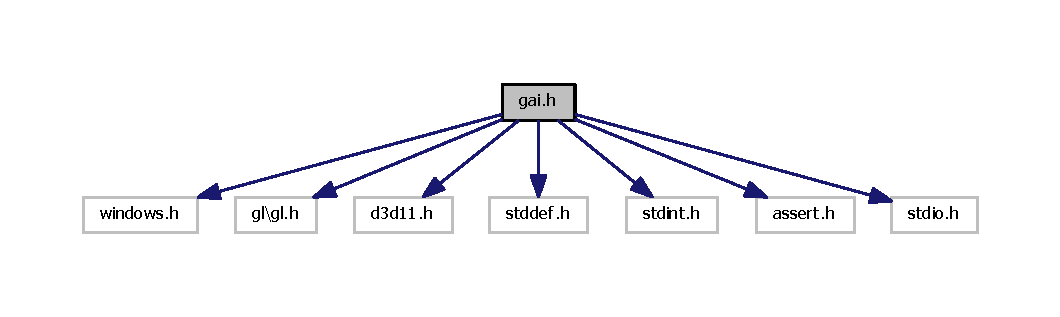
\includegraphics[width=350pt]{gai_8h__incl}
\end{center}
\end{figure}
This graph shows which files directly or indirectly include this file\+:\nopagebreak
\begin{figure}[H]
\begin{center}
\leavevmode
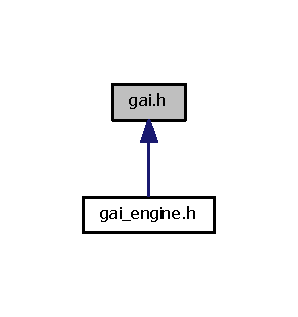
\includegraphics[width=143pt]{gai_8h__dep__incl}
\end{center}
\end{figure}
\subsection*{Classes}
\begin{DoxyCompactItemize}
\item 
struct \hyperlink{gai_8h_structgai__growable__header}{gai\+\_\+growable\+\_\+header}
\item 
struct \hyperlink{gai_8h_structgai__clock}{gai\+\_\+clock}
\item 
struct \hyperlink{gai_8h_structgai__file}{gai\+\_\+file}
\item 
union \hyperlink{gai_8h_uniongai__filetime}{gai\+\_\+filetime}
\item 
union \hyperlink{gai_8h_uniongai__filesize}{gai\+\_\+filesize}
\item 
struct \hyperlink{gai_8h_structgai__fileinfo}{gai\+\_\+fileinfo}
\item 
struct \hyperlink{gai_8h_structgai__window__callback}{gai\+\_\+window\+\_\+callback}
\item 
struct \hyperlink{structgai__window}{gai\+\_\+window}
\item 
union \hyperlink{structgai__window_uniongai__window_1_1_c_t_x}{gai\+\_\+window\+::\+C\+TX}
\item 
struct \hyperlink{structgai__window_structgai__window_1_1_c_t_x_1_1_o_p_e_n_g_l}{gai\+\_\+window\+::\+C\+T\+X\+::\+O\+P\+E\+N\+GL}
\item 
struct \hyperlink{structgai__window_structgai__window_1_1_c_t_x_1_1_d_i_r_e_c_t_x11}{gai\+\_\+window\+::\+C\+T\+X\+::\+D\+I\+R\+E\+C\+T\+X11}
\item 
struct \hyperlink{structgai__window_structgai__window_1_1_i_n_p_u_t}{gai\+\_\+window\+::\+I\+N\+P\+UT}
\item 
struct \hyperlink{gai_8h_structgai__filetime_8____unnamed____}{gai\+\_\+filetime.\+\_\+\+\_\+unnamed\+\_\+\+\_\+}
\item 
struct \hyperlink{gai_8h_structgai__filesize_8____unnamed____}{gai\+\_\+filesize.\+\_\+\+\_\+unnamed\+\_\+\+\_\+}
\end{DoxyCompactItemize}
\subsection*{Macros}
\begin{DoxyCompactItemize}
\item 
\mbox{\Hypertarget{gai_8h_a779f25f23ca7656b2c51f62beb0ddcd7}\label{gai_8h_a779f25f23ca7656b2c51f62beb0ddcd7}} 
\#define {\bfseries G\+A\+I\+\_\+\+O\+S\+\_\+\+R\+E\+S\+O\+L\+U\+T\+I\+ON}
\item 
\mbox{\Hypertarget{gai_8h_a41f9c5fb8b08eb5dc3edce4dcb37fee7}\label{gai_8h_a41f9c5fb8b08eb5dc3edce4dcb37fee7}} 
\#define {\bfseries true}~1
\item 
\mbox{\Hypertarget{gai_8h_a65e9886d74aaee76545e83dd09011727}\label{gai_8h_a65e9886d74aaee76545e83dd09011727}} 
\#define {\bfseries false}~0
\item 
\mbox{\Hypertarget{gai_8h_abc0bc067e1a88c12d70de5926e962368}\label{gai_8h_abc0bc067e1a88c12d70de5926e962368}} 
\#define {\bfseries G\+A\+I\+\_\+\+T\+Y\+P\+E\+D\+E\+FS}~1
\item 
\#define \hyperlink{gai_8h_a335a7d91cecb2b1e5745c06803bdf23a}{G\+A\+I\+\_\+\+D\+EF}~extern
\item 
\mbox{\Hypertarget{gai_8h_aeb3ca9c144e88d45449d54e515dc0dce}\label{gai_8h_aeb3ca9c144e88d45449d54e515dc0dce}} 
\#define {\bfseries G\+A\+I\+\_\+\+A\+S\+S\+E\+RT}(cond)~assert(cond)
\item 
\#define \hyperlink{gai_8h_a1acedd3479fb2a001b5f284e4de6b90e}{gai\+\_\+growable}(type)~type $\ast$
\item 
\mbox{\Hypertarget{gai_8h_af6553ddc52e978b3c13a65605c5a0a6c}\label{gai_8h_af6553ddc52e978b3c13a65605c5a0a6c}} 
\#define {\bfseries G\+A\+I\+\_\+\+G\+R\+O\+W\+A\+B\+L\+E\+\_\+\+G\+R\+O\+W\+\_\+\+S\+T\+R\+A\+T\+E\+GY}(x)~(((x)$\ast$2)+8)
\item 
\mbox{\Hypertarget{gai_8h_ae22d900ee344bfb945857eeb78b42b0b}\label{gai_8h_ae22d900ee344bfb945857eeb78b42b0b}} 
\#define {\bfseries G\+A\+I\+\_\+\+G\+R\+O\+W\+A\+B\+L\+E\+\_\+\+G\+E\+T\+\_\+\+H\+E\+A\+D\+ER}(x)~((\hyperlink{gai_8h_structgai__growable__header}{gai\+\_\+growable\+\_\+header}$\ast$)(x)-\/1)
\item 
\mbox{\Hypertarget{gai_8h_a8c72c7bd103b78930e2e237c9152d7dd}\label{gai_8h_a8c72c7bd103b78930e2e237c9152d7dd}} 
\#define {\bfseries gai\+\_\+growable\+\_\+count}(x)~(G\+A\+I\+\_\+\+G\+R\+O\+W\+A\+B\+L\+E\+\_\+\+G\+E\+T\+\_\+\+H\+E\+A\+D\+ER(x)-\/$>$count)
\item 
\mbox{\Hypertarget{gai_8h_a5410a25f633c6ac232d0e6d0f6a6f4c0}\label{gai_8h_a5410a25f633c6ac232d0e6d0f6a6f4c0}} 
\#define {\bfseries gai\+\_\+growable\+\_\+capacity}(x)~(G\+A\+I\+\_\+\+G\+R\+O\+W\+A\+B\+L\+E\+\_\+\+G\+E\+T\+\_\+\+H\+E\+A\+D\+ER(x)-\/$>$capacity)
\item 
\mbox{\Hypertarget{gai_8h_ad2016f2fe64172616fb67cf31ffe41e8}\label{gai_8h_ad2016f2fe64172616fb67cf31ffe41e8}} 
\#define {\bfseries gai\+\_\+growable\+\_\+clear}(x)~(G\+A\+I\+\_\+\+G\+R\+O\+W\+A\+B\+L\+E\+\_\+\+G\+E\+T\+\_\+\+H\+E\+A\+D\+ER(x)-\/$>$count = 0)
\item 
\#define {\bfseries gai\+\_\+growable\+\_\+init}(x)
\item 
\#define {\bfseries gai\+\_\+growable\+\_\+free}(x)
\item 
\#define {\bfseries gai\+\_\+growable\+\_\+append}(x,  item)
\item 
\#define {\bfseries gai\+\_\+growable\+\_\+append\+\_\+array}(x,  items,  item\+\_\+count)
\item 
\#define \hyperlink{gai_8h_ac28875a4f36c342fb6ab07be087428a7}{G\+A\+I\+\_\+\+S\+O\+R\+T\+\_\+\+C\+O\+M\+P\+A\+R\+E\+\_\+\+P\+R\+OC}(name)~int name(void const $\ast$a, void const $\ast$b)
\item 
\mbox{\Hypertarget{gai_8h_a52383b5393250964d2cd0a452cf68c93}\label{gai_8h_a52383b5393250964d2cd0a452cf68c93}} 
\#define {\bfseries gai\+\_\+sort\+\_\+array}(arr,  elements,  cmp\+\_\+fn)~gai\+\_\+sort((arr), (elements), sizeof($\ast$(arr)), cmp\+\_\+fn)
\item 
\mbox{\Hypertarget{gai_8h_a62a4d8b8a4b063264b85228bb45b0837}\label{gai_8h_a62a4d8b8a4b063264b85228bb45b0837}} 
\#define {\bfseries gai\+\_\+sort\+\_\+array\+\_\+i32}(arr,  elements)~gai\+\_\+sort((arr), (elements), sizeof(i32), \+\_\+\+\_\+gai\+\_\+i32\+\_\+cmp)
\item 
\mbox{\Hypertarget{gai_8h_a14f9b7fd10cdd558ae274ed659771a82}\label{gai_8h_a14f9b7fd10cdd558ae274ed659771a82}} 
\#define {\bfseries gai\+\_\+sort\+\_\+array\+\_\+i64}(arr,  elements)~gai\+\_\+sort((arr), (elements), sizeof(i64), \+\_\+\+\_\+gai\+\_\+i64\+\_\+cmp)
\item 
\mbox{\Hypertarget{gai_8h_a01f8e358d37bbd9fec27ac2cf10459b8}\label{gai_8h_a01f8e358d37bbd9fec27ac2cf10459b8}} 
\#define {\bfseries gai\+\_\+sort\+\_\+array\+\_\+r32}(arr,  elements)~gai\+\_\+sort((arr), (elements), sizeof(r32), \+\_\+\+\_\+gai\+\_\+r32\+\_\+cmp)
\item 
\mbox{\Hypertarget{gai_8h_a317f4820c5c2cd3f39c009a4471a8280}\label{gai_8h_a317f4820c5c2cd3f39c009a4471a8280}} 
\#define {\bfseries gai\+\_\+sort\+\_\+array\+\_\+r64}(arr,  elements)~gai\+\_\+sort((arr), (elements), sizeof(r64), \+\_\+\+\_\+gai\+\_\+r64\+\_\+cmp)
\end{DoxyCompactItemize}
\subsection*{Typedefs}
\begin{DoxyCompactItemize}
\item 
\mbox{\Hypertarget{gai_8h_a92c50087ca0e64fa93fc59402c55f8ca}\label{gai_8h_a92c50087ca0e64fa93fc59402c55f8ca}} 
typedef uint8\+\_\+t {\bfseries u8}
\item 
\mbox{\Hypertarget{gai_8h_ae3702327b5f47e83b431e22b33da7b58}\label{gai_8h_ae3702327b5f47e83b431e22b33da7b58}} 
typedef int8\+\_\+t {\bfseries i8}
\item 
\mbox{\Hypertarget{gai_8h_ace9d960e74685e2cd84b36132dbbf8aa}\label{gai_8h_ace9d960e74685e2cd84b36132dbbf8aa}} 
typedef uint16\+\_\+t {\bfseries u16}
\item 
\mbox{\Hypertarget{gai_8h_ad309dbcaeea13aa602d686964156ea0b}\label{gai_8h_ad309dbcaeea13aa602d686964156ea0b}} 
typedef int16\+\_\+t {\bfseries i16}
\item 
\mbox{\Hypertarget{gai_8h_afaa62991928fb9fb18ff0db62a040aba}\label{gai_8h_afaa62991928fb9fb18ff0db62a040aba}} 
typedef uint32\+\_\+t {\bfseries u32}
\item 
\mbox{\Hypertarget{gai_8h_a48d6cd8e4135fb2ff7e7f2dac84089ec}\label{gai_8h_a48d6cd8e4135fb2ff7e7f2dac84089ec}} 
typedef int32\+\_\+t {\bfseries i32}
\item 
\mbox{\Hypertarget{gai_8h_aafa04bc3cb166e826b75a23f4add4b59}\label{gai_8h_aafa04bc3cb166e826b75a23f4add4b59}} 
typedef float {\bfseries r32}
\item 
\mbox{\Hypertarget{gai_8h_a3f7e2bcbb0b4c338f3c4f6c937cd4234}\label{gai_8h_a3f7e2bcbb0b4c338f3c4f6c937cd4234}} 
typedef uint64\+\_\+t {\bfseries u64}
\item 
\mbox{\Hypertarget{gai_8h_a85cb35fbe5bf2961d7ad5f26814a91a2}\label{gai_8h_a85cb35fbe5bf2961d7ad5f26814a91a2}} 
typedef int64\+\_\+t {\bfseries i64}
\item 
\mbox{\Hypertarget{gai_8h_af3fb0780dd5bc8ff8740028f077610e7}\label{gai_8h_af3fb0780dd5bc8ff8740028f077610e7}} 
typedef double {\bfseries r64}
\item 
\mbox{\Hypertarget{gai_8h_a9d1a1d99b6972446ae039de3d9599b96}\label{gai_8h_a9d1a1d99b6972446ae039de3d9599b96}} 
typedef int32\+\_\+t {\bfseries b32}
\item 
\mbox{\Hypertarget{gai_8h_a2a7256d9664d3dc9c9b2edf2d04f2c53}\label{gai_8h_a2a7256d9664d3dc9c9b2edf2d04f2c53}} 
typedef u8 {\bfseries gai\+\_\+key\+\_\+state}
\item 
\mbox{\Hypertarget{gai_8h_a9a839bb0a3523c7b93b73f6440acbbb1}\label{gai_8h_a9a839bb0a3523c7b93b73f6440acbbb1}} 
typedef void {\bfseries gai\+\_\+window\+\_\+input\+\_\+callback}(i32 key, u8 state)
\end{DoxyCompactItemize}
\subsection*{Enumerations}
\begin{DoxyCompactItemize}
\item 
enum \hyperlink{gai_8h_a157d385f60e2ae934dc7854ae787ee44}{gai\+\_\+window\+\_\+flags} \{ \newline
{\bfseries gai\+Window\+Flags\+None} = 0x00, 
\hyperlink{gai_8h_a157d385f60e2ae934dc7854ae787ee44a51e1f5f38bf0c41063c43c6fd5afe26d}{gai\+Window\+Flags\+Minimized} = 0x01, 
\hyperlink{gai_8h_a157d385f60e2ae934dc7854ae787ee44adeacefd22a411eaf0e25ee9b072f9da6}{gai\+Window\+Flags\+Maximized} = 0x02, 
\hyperlink{gai_8h_a157d385f60e2ae934dc7854ae787ee44a5269cdd41791072e9383c3758d5d87d6}{gai\+Window\+Flags\+Borderless} = 0x04, 
\newline
\hyperlink{gai_8h_a157d385f60e2ae934dc7854ae787ee44ade455488dffb8dca918636a11ebad5dd}{gai\+Window\+Flags\+Fullscreen} = 0x10
 \}
\item 
\mbox{\Hypertarget{gai_8h_a9a29214276d175d59c57b660801d8015}\label{gai_8h_a9a29214276d175d59c57b660801d8015}} 
enum {\bfseries gai\+\_\+renderer\+\_\+type} \{ {\bfseries gai\+Renderer\+Default}, 
{\bfseries gai\+Renderer\+D\+X11}, 
{\bfseries gai\+Renderer\+Open\+GL}, 
{\bfseries gai\+Renderer\+Count}
 \}
\item 
\mbox{\Hypertarget{gai_8h_a7917ae9cf8fe8da8c07dc2239574a45d}\label{gai_8h_a7917ae9cf8fe8da8c07dc2239574a45d}} 
enum {\bfseries gai\+\_\+mouse\+\_\+button} \{ \newline
{\bfseries gai\+Mouse\+Left}, 
{\bfseries gai\+Mouse\+Middle}, 
{\bfseries gai\+Mouse\+Right}, 
{\bfseries gai\+Mouse\+Extra1}, 
\newline
{\bfseries gai\+Mouse\+Extra2}
 \}
\item 
\mbox{\Hypertarget{gai_8h_a924104711ebf4eea20e17e8795d61a9d}\label{gai_8h_a924104711ebf4eea20e17e8795d61a9d}} 
enum {\bfseries gai\+\_\+key\+\_\+state\+\_\+enum} \{ {\bfseries gai\+Keystate\+Down} = 0x1, 
{\bfseries gai\+Keystate\+Pressed} = 0x2, 
{\bfseries gai\+Keystate\+Released} = 0x4
 \}
\item 
\mbox{\Hypertarget{gai_8h_ad8ecbc8c48164e83ea61c31197b0332a}\label{gai_8h_ad8ecbc8c48164e83ea61c31197b0332a}} 
enum {\bfseries gai\+\_\+callback\+\_\+type\+\_\+enum} \{ {\bfseries gai\+Unhandled\+Event} = 0x0, 
{\bfseries gai\+Input\+Event} = 0x1
 \}
\end{DoxyCompactItemize}
\subsection*{Functions}
\begin{DoxyCompactItemize}
\item 
void \hyperlink{gai_8h_aa02d51324b115958d15b739432c9695d}{gai\+\_\+memswap} (u8 $\ast$a, u8 $\ast$b, size\+\_\+t size)
\item 
\mbox{\Hypertarget{gai_8h_af09298232799c623b93bcff3ca8562c4}\label{gai_8h_af09298232799c623b93bcff3ca8562c4}} 
void $\ast$ {\bfseries gai\+\_\+growable\+\_\+grow} (void $\ast$array, size\+\_\+t new\+\_\+capacity, size\+\_\+t element\+\_\+size)
\item 
\mbox{\Hypertarget{gai_8h_ac88d203d35eba85a32b0eaa10617e29e}\label{gai_8h_ac88d203d35eba85a32b0eaa10617e29e}} 
typedef {\bfseries G\+A\+I\+\_\+\+S\+O\+R\+T\+\_\+\+C\+O\+M\+P\+A\+R\+E\+\_\+\+P\+R\+OC} (gai\+\_\+sort\+\_\+compare\+\_\+fn)
\item 
\mbox{\Hypertarget{gai_8h_a7b9bcec1c651acfd3284f5373eb2b5a5}\label{gai_8h_a7b9bcec1c651acfd3284f5373eb2b5a5}} 
\hyperlink{gai_8h_a335a7d91cecb2b1e5745c06803bdf23a}{G\+A\+I\+\_\+\+D\+EF} void {\bfseries gai\+\_\+sort} (void $\ast$array, size\+\_\+t elements, size\+\_\+t element\+\_\+size, gai\+\_\+sort\+\_\+compare\+\_\+fn cmp)
\item 
\mbox{\Hypertarget{gai_8h_aad42663f47feda07b05dad333fa8eaab}\label{gai_8h_aad42663f47feda07b05dad333fa8eaab}} 
\hyperlink{gai_8h_a335a7d91cecb2b1e5745c06803bdf23a}{G\+A\+I\+\_\+\+D\+EF} \hyperlink{gai_8h_structgai__clock}{gai\+\_\+clock} {\bfseries gai\+\_\+clock\+\_\+init} ()
\item 
\mbox{\Hypertarget{gai_8h_af560ae2c4195ca5e7859380435afd013}\label{gai_8h_af560ae2c4195ca5e7859380435afd013}} 
\hyperlink{gai_8h_a335a7d91cecb2b1e5745c06803bdf23a}{G\+A\+I\+\_\+\+D\+EF} r64 {\bfseries gai\+\_\+clock\+\_\+get} (\hyperlink{gai_8h_structgai__clock}{gai\+\_\+clock} $\ast$clock)
\item 
\mbox{\Hypertarget{gai_8h_acc242c4caa720d7c754b3c11a6d7b70d}\label{gai_8h_acc242c4caa720d7c754b3c11a6d7b70d}} 
\hyperlink{gai_8h_a335a7d91cecb2b1e5745c06803bdf23a}{G\+A\+I\+\_\+\+D\+EF} \hyperlink{gai_8h_structgai__file}{gai\+\_\+file} {\bfseries gai\+\_\+file\+\_\+open} (const char $\ast$filename, const char $\ast$mode)
\item 
\mbox{\Hypertarget{gai_8h_a95e48873b97b236f57dde64e83b061ff}\label{gai_8h_a95e48873b97b236f57dde64e83b061ff}} 
\hyperlink{gai_8h_a335a7d91cecb2b1e5745c06803bdf23a}{G\+A\+I\+\_\+\+D\+EF} size\+\_\+t {\bfseries gai\+\_\+file\+\_\+write} (\hyperlink{gai_8h_structgai__file}{gai\+\_\+file} $\ast$file, void $\ast$data, size\+\_\+t length)
\item 
\mbox{\Hypertarget{gai_8h_a6d58326c4657cf1bd5e2e4b4f6cd0bec}\label{gai_8h_a6d58326c4657cf1bd5e2e4b4f6cd0bec}} 
\hyperlink{gai_8h_a335a7d91cecb2b1e5745c06803bdf23a}{G\+A\+I\+\_\+\+D\+EF} size\+\_\+t {\bfseries gai\+\_\+file\+\_\+read} (\hyperlink{gai_8h_structgai__file}{gai\+\_\+file} $\ast$file, void $\ast$buffer, size\+\_\+t bytes\+\_\+to\+\_\+read, i32 offset)
\item 
\mbox{\Hypertarget{gai_8h_ad582bab01279c72c5a1b51b84e25fca7}\label{gai_8h_ad582bab01279c72c5a1b51b84e25fca7}} 
\hyperlink{gai_8h_a335a7d91cecb2b1e5745c06803bdf23a}{G\+A\+I\+\_\+\+D\+EF} size\+\_\+t {\bfseries gai\+\_\+file\+\_\+read\+\_\+all} (\hyperlink{gai_8h_structgai__file}{gai\+\_\+file} $\ast$file, void $\ast$buffer)
\item 
\mbox{\Hypertarget{gai_8h_aa38b6f0895fff1d1f81f8e71fa0b42d3}\label{gai_8h_aa38b6f0895fff1d1f81f8e71fa0b42d3}} 
\hyperlink{gai_8h_a335a7d91cecb2b1e5745c06803bdf23a}{G\+A\+I\+\_\+\+D\+EF} void {\bfseries gai\+\_\+file\+\_\+close} (\hyperlink{gai_8h_structgai__file}{gai\+\_\+file} $\ast$file)
\item 
\mbox{\Hypertarget{gai_8h_abbe50fe46424202d10e727549d790900}\label{gai_8h_abbe50fe46424202d10e727549d790900}} 
\hyperlink{gai_8h_a335a7d91cecb2b1e5745c06803bdf23a}{G\+A\+I\+\_\+\+D\+EF} b32 {\bfseries gai\+\_\+file\+\_\+exists} (const char $\ast$filename)
\item 
\mbox{\Hypertarget{gai_8h_ae522af434bcfa8029fe46f0e5f9e90d5}\label{gai_8h_ae522af434bcfa8029fe46f0e5f9e90d5}} 
\hyperlink{gai_8h_a335a7d91cecb2b1e5745c06803bdf23a}{G\+A\+I\+\_\+\+D\+EF} \hyperlink{gai_8h_structgai__fileinfo}{gai\+\_\+fileinfo} {\bfseries gai\+\_\+file\+\_\+getinfo} (const char $\ast$filename)
\item 
\mbox{\Hypertarget{gai_8h_a74b18b0b489ca0d9c827cdc873eff87b}\label{gai_8h_a74b18b0b489ca0d9c827cdc873eff87b}} 
\hyperlink{gai_8h_a335a7d91cecb2b1e5745c06803bdf23a}{G\+A\+I\+\_\+\+D\+EF} i32 {\bfseries gai\+\_\+window\+\_\+init} (\hyperlink{structgai__window}{gai\+\_\+window} $\ast$window, const char $\ast$title, i32 width, i32 height, u32 flags)
\item 
\mbox{\Hypertarget{gai_8h_aa915b135dfb1bc12b51c10d7dc4e0e8c}\label{gai_8h_aa915b135dfb1bc12b51c10d7dc4e0e8c}} 
\hyperlink{gai_8h_a335a7d91cecb2b1e5745c06803bdf23a}{G\+A\+I\+\_\+\+D\+EF} i32 {\bfseries gai\+\_\+window\+\_\+init\+\_\+gl} (\hyperlink{structgai__window}{gai\+\_\+window} $\ast$window, const char $\ast$title, i32 width, i32 height, u32 flags, i32 minor, i32 major, b32 core\+\_\+profile, b32 debug)
\item 
\mbox{\Hypertarget{gai_8h_ac08dcf962361fe69a25baf8dc212c1a5}\label{gai_8h_ac08dcf962361fe69a25baf8dc212c1a5}} 
\hyperlink{gai_8h_a335a7d91cecb2b1e5745c06803bdf23a}{G\+A\+I\+\_\+\+D\+EF} i32 {\bfseries gai\+\_\+window\+\_\+init\+\_\+dx} (\hyperlink{structgai__window}{gai\+\_\+window} $\ast$window, const char $\ast$title, i32 width, i32 height, u32 flags)
\item 
\mbox{\Hypertarget{gai_8h_ac1bf3ce3bcef7ed6f0bcccb9f8e55906}\label{gai_8h_ac1bf3ce3bcef7ed6f0bcccb9f8e55906}} 
\hyperlink{gai_8h_a335a7d91cecb2b1e5745c06803bdf23a}{G\+A\+I\+\_\+\+D\+EF} i32 {\bfseries gai\+\_\+window\+\_\+destroy} (\hyperlink{structgai__window}{gai\+\_\+window} $\ast$window)
\item 
\mbox{\Hypertarget{gai_8h_a71b19503c53dff4f70132cc96677ce17}\label{gai_8h_a71b19503c53dff4f70132cc96677ce17}} 
\hyperlink{gai_8h_a335a7d91cecb2b1e5745c06803bdf23a}{G\+A\+I\+\_\+\+D\+EF} void {\bfseries gai\+\_\+window\+\_\+vsync} (\hyperlink{structgai__window}{gai\+\_\+window} $\ast$window, b32 state)
\item 
\mbox{\Hypertarget{gai_8h_a4d71a8be3cdb258f5950817dabaeb7ef}\label{gai_8h_a4d71a8be3cdb258f5950817dabaeb7ef}} 
\hyperlink{gai_8h_a335a7d91cecb2b1e5745c06803bdf23a}{G\+A\+I\+\_\+\+D\+EF} b32 {\bfseries gai\+\_\+window\+\_\+vsync\+\_\+enabled} (\hyperlink{structgai__window}{gai\+\_\+window} $\ast$window)
\item 
\mbox{\Hypertarget{gai_8h_a2780b47a6e66338ec820f2e55dc3a172}\label{gai_8h_a2780b47a6e66338ec820f2e55dc3a172}} 
\hyperlink{gai_8h_a335a7d91cecb2b1e5745c06803bdf23a}{G\+A\+I\+\_\+\+D\+EF} void {\bfseries gai\+\_\+window\+\_\+handle\+\_\+messages} (\hyperlink{structgai__window}{gai\+\_\+window} $\ast$window, b32 block)
\item 
\mbox{\Hypertarget{gai_8h_a1b9a78ec80c1195f0a65da06c36d0976}\label{gai_8h_a1b9a78ec80c1195f0a65da06c36d0976}} 
\hyperlink{gai_8h_a335a7d91cecb2b1e5745c06803bdf23a}{G\+A\+I\+\_\+\+D\+EF} void {\bfseries gai\+\_\+window\+\_\+display} (\hyperlink{structgai__window}{gai\+\_\+window} $\ast$window)
\item 
\mbox{\Hypertarget{gai_8h_ad5c49787af9602418dddff1f1a2c8be9}\label{gai_8h_ad5c49787af9602418dddff1f1a2c8be9}} 
\hyperlink{gai_8h_a335a7d91cecb2b1e5745c06803bdf23a}{G\+A\+I\+\_\+\+D\+EF} void {\bfseries gai\+\_\+window\+\_\+show} (\hyperlink{structgai__window}{gai\+\_\+window} $\ast$window)
\item 
\mbox{\Hypertarget{gai_8h_ac80f28c417a19209b074b263c382da36}\label{gai_8h_ac80f28c417a19209b074b263c382da36}} 
\hyperlink{gai_8h_a335a7d91cecb2b1e5745c06803bdf23a}{G\+A\+I\+\_\+\+D\+EF} void {\bfseries gai\+\_\+window\+\_\+hide} (\hyperlink{structgai__window}{gai\+\_\+window} $\ast$window)
\item 
\mbox{\Hypertarget{gai_8h_a1211bfbe9d14ccc70e7272c8a2090276}\label{gai_8h_a1211bfbe9d14ccc70e7272c8a2090276}} 
\hyperlink{gai_8h_a335a7d91cecb2b1e5745c06803bdf23a}{G\+A\+I\+\_\+\+D\+EF} b32 {\bfseries gai\+\_\+window\+\_\+set\+\_\+foreground} (\hyperlink{structgai__window}{gai\+\_\+window} $\ast$window)
\item 
\mbox{\Hypertarget{gai_8h_a8f53031dfe738cc41d8f89466447d32e}\label{gai_8h_a8f53031dfe738cc41d8f89466447d32e}} 
\hyperlink{gai_8h_a335a7d91cecb2b1e5745c06803bdf23a}{G\+A\+I\+\_\+\+D\+EF} b32 {\bfseries gai\+\_\+window\+\_\+is\+\_\+foreground} (\hyperlink{structgai__window}{gai\+\_\+window} $\ast$window)
\item 
\mbox{\Hypertarget{gai_8h_a4b164149785308f03774a60fcb264554}\label{gai_8h_a4b164149785308f03774a60fcb264554}} 
\hyperlink{gai_8h_a335a7d91cecb2b1e5745c06803bdf23a}{G\+A\+I\+\_\+\+D\+EF} void {\bfseries gai\+\_\+window\+\_\+set\+\_\+position} (\hyperlink{structgai__window}{gai\+\_\+window} $\ast$window, i32 x, i32 y)
\item 
\mbox{\Hypertarget{gai_8h_aba36a83b8437a1ec7a3a899fae3a02ec}\label{gai_8h_aba36a83b8437a1ec7a3a899fae3a02ec}} 
\hyperlink{gai_8h_a335a7d91cecb2b1e5745c06803bdf23a}{G\+A\+I\+\_\+\+D\+EF} void {\bfseries gai\+\_\+window\+\_\+borderless} (\hyperlink{structgai__window}{gai\+\_\+window} $\ast$window, b32 state)
\item 
\mbox{\Hypertarget{gai_8h_ae003c1dc1301bbcf9ab94c2abfe8dcf5}\label{gai_8h_ae003c1dc1301bbcf9ab94c2abfe8dcf5}} 
\hyperlink{gai_8h_a335a7d91cecb2b1e5745c06803bdf23a}{G\+A\+I\+\_\+\+D\+EF} void {\bfseries gai\+\_\+window\+\_\+register\+\_\+callback} (\hyperlink{structgai__window}{gai\+\_\+window} $\ast$window, gai\+\_\+callback\+\_\+type\+\_\+enum type, void $\ast$callback)
\item 
\mbox{\Hypertarget{gai_8h_a72b08fd434590118b949212e5e3b6199}\label{gai_8h_a72b08fd434590118b949212e5e3b6199}} 
\hyperlink{gai_8h_a335a7d91cecb2b1e5745c06803bdf23a}{G\+A\+I\+\_\+\+D\+EF} void {\bfseries gai\+\_\+window\+\_\+unregister\+\_\+callback} (\hyperlink{structgai__window}{gai\+\_\+window} $\ast$window, void $\ast$callback)
\item 
\mbox{\Hypertarget{gai_8h_a8b00f5c92eba88e860faf7e41eb54680}\label{gai_8h_a8b00f5c92eba88e860faf7e41eb54680}} 
\hyperlink{gai_8h_a335a7d91cecb2b1e5745c06803bdf23a}{G\+A\+I\+\_\+\+D\+EF} b32 {\bfseries gai\+\_\+key\+\_\+down} (\hyperlink{structgai__window}{gai\+\_\+window} $\ast$window, i32 key)
\item 
\mbox{\Hypertarget{gai_8h_ab357cabb11019a790466a99494b8ee9e}\label{gai_8h_ab357cabb11019a790466a99494b8ee9e}} 
\hyperlink{gai_8h_a335a7d91cecb2b1e5745c06803bdf23a}{G\+A\+I\+\_\+\+D\+EF} b32 {\bfseries gai\+\_\+key\+\_\+released} (\hyperlink{structgai__window}{gai\+\_\+window} $\ast$window, i32 key)
\item 
\mbox{\Hypertarget{gai_8h_a2c9672c6544607970531970667f9ba0c}\label{gai_8h_a2c9672c6544607970531970667f9ba0c}} 
\hyperlink{gai_8h_a335a7d91cecb2b1e5745c06803bdf23a}{G\+A\+I\+\_\+\+D\+EF} b32 {\bfseries gai\+\_\+key\+\_\+pressed} (\hyperlink{structgai__window}{gai\+\_\+window} $\ast$window, i32 key)
\item 
\mbox{\Hypertarget{gai_8h_a38f0bb922bf4ba1465b54f91056fee26}\label{gai_8h_a38f0bb922bf4ba1465b54f91056fee26}} 
\hyperlink{gai_8h_a335a7d91cecb2b1e5745c06803bdf23a}{G\+A\+I\+\_\+\+D\+EF} b32 {\bfseries gai\+\_\+mouse\+\_\+down} (\hyperlink{structgai__window}{gai\+\_\+window} $\ast$window, i32 btnid)
\item 
\mbox{\Hypertarget{gai_8h_a7d5ec449d3810e49869e188a2c70031c}\label{gai_8h_a7d5ec449d3810e49869e188a2c70031c}} 
\hyperlink{gai_8h_a335a7d91cecb2b1e5745c06803bdf23a}{G\+A\+I\+\_\+\+D\+EF} b32 {\bfseries gai\+\_\+mouse\+\_\+released} (\hyperlink{structgai__window}{gai\+\_\+window} $\ast$window, i32 btnid)
\item 
\mbox{\Hypertarget{gai_8h_a2bc4940f8086396ce917131a0c14412b}\label{gai_8h_a2bc4940f8086396ce917131a0c14412b}} 
\hyperlink{gai_8h_a335a7d91cecb2b1e5745c06803bdf23a}{G\+A\+I\+\_\+\+D\+EF} b32 {\bfseries gai\+\_\+mouse\+\_\+pressed} (\hyperlink{structgai__window}{gai\+\_\+window} $\ast$window, i32 btnid)
\end{DoxyCompactItemize}


\subsection{Detailed Description}
designed as a cross platform single include header file for the most necessary features (window, dynamic array, qsort, network) 

{\bfseries Depends on the specific OS libraries and the standard c library} \begin{DoxyAuthor}{Author}
Andreas Gaida 
\end{DoxyAuthor}
\begin{DoxyDate}{Date}
23.\+05.\+2017 
\end{DoxyDate}


\subsection{Class Documentation}
\index{gai\+\_\+growable\+\_\+header@{gai\+\_\+growable\+\_\+header}}\label{structgai__growable__header}
\Hypertarget{gai_8h_structgai__growable__header}
\subsubsection{struct gai\+\_\+growable\+\_\+header}
\begin{DoxyFields}{Class Members}
\mbox{\Hypertarget{gai_8h_a2c34cb03293511a0c60a94a6681f210a}\label{gai_8h_a2c34cb03293511a0c60a94a6681f210a}} 
size\_t&
capacity&
\\
\hline

\mbox{\Hypertarget{gai_8h_a4ada9b200324f877f22c4bf53ee50a0e}\label{gai_8h_a4ada9b200324f877f22c4bf53ee50a0e}} 
size\_t&
count&
\\
\hline

\end{DoxyFields}
\index{gai\+\_\+clock@{gai\+\_\+clock}}\label{structgai__clock}
\Hypertarget{gai_8h_structgai__clock}
\subsubsection{struct gai\+\_\+clock}
time api



 $\vert$ $\vert$ $\vert$ $\vert$ $\vert$ $\vert$\+\_\+\+\_\+\+\_\+\+\_\+\+\_\+\+\_\+ $\vert$\+\_\+\+\_\+\+\_\+\+\_\+\+\_\+$\vert$ $\vert$\+\_\+\+\_\+\+\_\+\+\_\+\+\_\+\mbox{]} $\vert$ $\vert$ \+\_\+\+\_\+$\vert$\+\_\+\+\_\+ $\vert$ $\vert$ $\vert$ $\vert$\+\_\+\+\_\+\+\_\+\+\_\+\+\_\+\+\_\+ $\vert$ $\vert$ $\vert$ \+\_\+\+\_\+$\vert$\+\_\+\+\_\+ \begin{DoxyFields}{Class Members}
\mbox{\Hypertarget{gai_8h_ac5b1c8faa4ba4ea64abbf0250f39fb3b}\label{gai_8h_ac5b1c8faa4ba4ea64abbf0250f39fb3b}} 
r64&
frequency&
\\
\hline

\mbox{\Hypertarget{gai_8h_a0c256402d36ae426f60a816936a5cbd0}\label{gai_8h_a0c256402d36ae426f60a816936a5cbd0}} 
r64&
last\_clock&
\\
\hline

\end{DoxyFields}
\index{gai\+\_\+file@{gai\+\_\+file}}\label{structgai__file}
\Hypertarget{gai_8h_structgai__file}
\subsubsection{struct gai\+\_\+file}
file management api



 $\vert$\+\_\+\+\_\+\+\_\+\+\_\+\+\_\+\+\_\+ $\vert$ $\vert$ $\vert$\+\_\+\+\_\+\+\_\+\+\_\+\+\_\+\+\_\+ $\vert$\+\_\+\+\_\+\+\_\+\+\_\+\+\_\+$\vert$ $\vert$\+\_\+\+\_\+\+\_\+\+\_\+\+\_\+\mbox{]} $\vert$ $\vert$ \+\_\+\+\_\+$\vert$\+\_\+\+\_\+ $\vert$\+\_\+\+\_\+\+\_\+\+\_\+\+\_\+ $\vert$\+\_\+\+\_\+\+\_\+\+\_\+\+\_\+\+\_\+ $\vert$ $\vert$ $\vert$ \+\_\+\+\_\+$\vert$\+\_\+\+\_\+

For all of these functions the user has to provide the buffer. No memory allocation is happening in here! 
\begin{DoxyCode}
\hyperlink{gai_8h_structgai__file}{gai\_file} f = gai\_file\_open(\textcolor{stringliteral}{"mytest.txt"}, \textcolor{stringliteral}{"rb"});
\{
    u8 *buffer = (u8*) malloc(f.size + 1);
    i32 read\_bytes = gai\_file\_read\_all(&f, buffer);
    buffer[read\_bytes] = 0;
    free(buffer);
\}
\end{DoxyCode}
 \begin{DoxyFields}{Class Members}
\mbox{\Hypertarget{gai_8h_ad56695ce19bc1ed60d5c5b922d5ddf9f}\label{gai_8h_ad56695ce19bc1ed60d5c5b922d5ddf9f}} 
FILE $\ast$&
fp&
\\
\hline

\mbox{\Hypertarget{gai_8h_af9a348ebc291e2314db8d411eff252c4}\label{gai_8h_af9a348ebc291e2314db8d411eff252c4}} 
size\_t&
size&
\\
\hline

\end{DoxyFields}
\index{gai\+\_\+filetime@{gai\+\_\+filetime}}\label{uniongai__filetime}
\Hypertarget{gai_8h_uniongai__filetime}
\subsubsection{union gai\+\_\+filetime}
\begin{DoxyFields}{Class Members}
\mbox{\Hypertarget{gai_8h_a81ee39aa0aa1e4e5933cf1f16ef04c3e}\label{gai_8h_a81ee39aa0aa1e4e5933cf1f16ef04c3e}} 
struct \hyperlink{gai_8h_structgai__filetime_8____unnamed____}{gai\_filetime}&
\_\_unnamed\_\_&
\\
\hline

\mbox{\Hypertarget{gai_8h_a4c2845b575bfc8c90c06b6211c9c9314}\label{gai_8h_a4c2845b575bfc8c90c06b6211c9c9314}} 
i64&
time&
\\
\hline

\end{DoxyFields}
\index{gai\+\_\+filesize@{gai\+\_\+filesize}}\label{uniongai__filesize}
\Hypertarget{gai_8h_uniongai__filesize}
\subsubsection{union gai\+\_\+filesize}
\begin{DoxyFields}{Class Members}
\mbox{\Hypertarget{gai_8h_add5e278e3cd49bf7bc9416e7b6ca5fbe}\label{gai_8h_add5e278e3cd49bf7bc9416e7b6ca5fbe}} 
struct \hyperlink{gai_8h_structgai__filesize_8____unnamed____}{gai\_filesize}&
\_\_unnamed\_\_&
\\
\hline

\mbox{\Hypertarget{gai_8h_ae9d3b212e3398ec6af40665a6612d1e0}\label{gai_8h_ae9d3b212e3398ec6af40665a6612d1e0}} 
i64&
size&
\\
\hline

\end{DoxyFields}
\index{gai\+\_\+fileinfo@{gai\+\_\+fileinfo}}\label{structgai__fileinfo}
\Hypertarget{gai_8h_structgai__fileinfo}
\subsubsection{struct gai\+\_\+fileinfo}


Collaboration diagram for gai\+\_\+fileinfo\+:\nopagebreak
\begin{figure}[H]
\begin{center}
\leavevmode
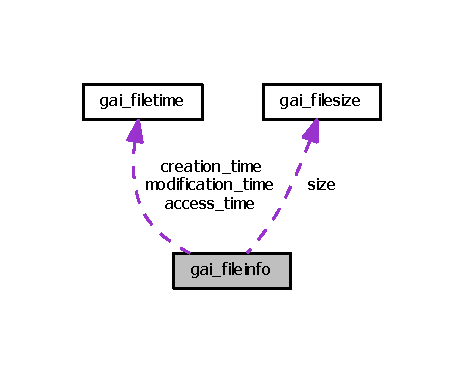
\includegraphics[width=223pt]{structgai__fileinfo__coll__graph}
\end{center}
\end{figure}
\begin{DoxyFields}{Class Members}
\mbox{\Hypertarget{gai_8h_a33e252c7ee367aedb5656e56f2565fa4}\label{gai_8h_a33e252c7ee367aedb5656e56f2565fa4}} 
\hyperlink{gai_8h_uniongai__filetime}{gai\_filetime}&
access\_time&
\\
\hline

\mbox{\Hypertarget{gai_8h_a8dbcbec051863fe8fd5e89d9b6140616}\label{gai_8h_a8dbcbec051863fe8fd5e89d9b6140616}} 
i32&
attributes&
\\
\hline

\mbox{\Hypertarget{gai_8h_a90d81f2fbc3fef3e335491a1c683019f}\label{gai_8h_a90d81f2fbc3fef3e335491a1c683019f}} 
\hyperlink{gai_8h_uniongai__filetime}{gai\_filetime}&
creation\_time&
\\
\hline

\mbox{\Hypertarget{gai_8h_af920e342a1fb82c9bf022e2b94b2e74e}\label{gai_8h_af920e342a1fb82c9bf022e2b94b2e74e}} 
\hyperlink{gai_8h_uniongai__filetime}{gai\_filetime}&
modification\_time&
\\
\hline

\mbox{\Hypertarget{gai_8h_a4bc6cf589dac9c3f29d096557630f27c}\label{gai_8h_a4bc6cf589dac9c3f29d096557630f27c}} 
\hyperlink{gai_8h_uniongai__filesize}{gai\_filesize}&
size&
\\
\hline

\end{DoxyFields}
\index{gai\+\_\+window\+\_\+callback@{gai\+\_\+window\+\_\+callback}}\label{structgai__window__callback}
\Hypertarget{gai_8h_structgai__window__callback}
\subsubsection{struct gai\+\_\+window\+\_\+callback}
\begin{DoxyFields}{Class Members}
\mbox{\Hypertarget{gai_8h_a2f106c6d1bd60b5ffd71630b9695019a}\label{gai_8h_a2f106c6d1bd60b5ffd71630b9695019a}} 
void $\ast$&
callback&
\\
\hline

\mbox{\Hypertarget{gai_8h_ac1ce8e0a7eecf5066151b7801c8b0e5e}\label{gai_8h_ac1ce8e0a7eecf5066151b7801c8b0e5e}} 
u16&
type&
\\
\hline

\end{DoxyFields}
\index{gai\+\_\+window\+::\+C\+TX@{gai\+\_\+window\+::\+C\+TX}}\label{uniongai__window_1_1_c_t_x}
\Hypertarget{structgai__window_uniongai__window_1_1_c_t_x}
\subsubsection{union gai\+\_\+window\+:\+:C\+TX}


Collaboration diagram for gai\+\_\+window\+:\+:C\+TX\+:
\nopagebreak
\begin{figure}[H]
\begin{center}
\leavevmode
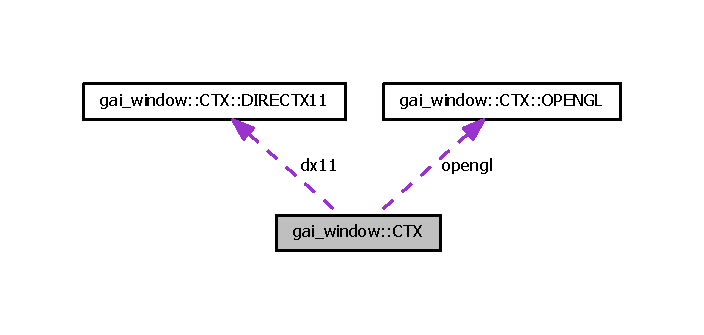
\includegraphics[width=338pt]{uniongai__window_1_1_c_t_x__coll__graph}
\end{center}
\end{figure}
\begin{DoxyFields}{Class Members}
\mbox{\Hypertarget{structgai__window_a2112189a9a1bc9b668a7c75a5527a52d}\label{structgai__window_a2112189a9a1bc9b668a7c75a5527a52d}} 
struct \hyperlink{structgai__window_structgai__window_1_1_c_t_x_1_1_d_i_r_e_c_t_x11}{DIRECTX11}&
dx11&
\\
\hline

\mbox{\Hypertarget{structgai__window_a2b95d5e69bdf2e65fa3bafc4061d0ec7}\label{structgai__window_a2b95d5e69bdf2e65fa3bafc4061d0ec7}} 
struct \hyperlink{structgai__window_structgai__window_1_1_c_t_x_1_1_o_p_e_n_g_l}{OPENGL}&
opengl&
\\
\hline

\end{DoxyFields}
\index{gai\+\_\+window\+::\+C\+T\+X\+::\+O\+P\+E\+N\+GL@{gai\+\_\+window\+::\+C\+T\+X\+::\+O\+P\+E\+N\+GL}}\label{structgai__window_1_1_c_t_x_1_1_o_p_e_n_g_l}
\Hypertarget{structgai__window_structgai__window_1_1_c_t_x_1_1_o_p_e_n_g_l}
\subsubsection{struct gai\+\_\+window\+:\+:C\+TX\+:\+:O\+P\+E\+N\+GL}
\begin{DoxyFields}{Class Members}
\mbox{\Hypertarget{structgai__window_ada16321f77bce8bf810b71ac857c6895}\label{structgai__window_ada16321f77bce8bf810b71ac857c6895}} 
void $\ast$&
context&
\\
\hline

\mbox{\Hypertarget{structgai__window_ac868cfbd6dde9272fb2935f7d52bf467}\label{structgai__window_ac868cfbd6dde9272fb2935f7d52bf467}} 
i32&
core&
\\
\hline

\mbox{\Hypertarget{structgai__window_a0db9760ca37f00fd313884a70ebd7bc8}\label{structgai__window_a0db9760ca37f00fd313884a70ebd7bc8}} 
i32&
debug&
\\
\hline

\mbox{\Hypertarget{structgai__window_a68cdd80ef3e595a05cac2120660ae735}\label{structgai__window_a68cdd80ef3e595a05cac2120660ae735}} 
i32&
major&
\\
\hline

\mbox{\Hypertarget{structgai__window_a7f9d61b341b6103e00132c70fcad72d9}\label{structgai__window_a7f9d61b341b6103e00132c70fcad72d9}} 
i32&
minor&
\\
\hline

\end{DoxyFields}
\index{gai\+\_\+window\+::\+C\+T\+X\+::\+D\+I\+R\+E\+C\+T\+X11@{gai\+\_\+window\+::\+C\+T\+X\+::\+D\+I\+R\+E\+C\+T\+X11}}\label{structgai__window_1_1_c_t_x_1_1_d_i_r_e_c_t_x11}
\Hypertarget{structgai__window_structgai__window_1_1_c_t_x_1_1_d_i_r_e_c_t_x11}
\subsubsection{struct gai\+\_\+window\+:\+:C\+TX\+:\+:D\+I\+R\+E\+C\+T\+X11}
\begin{DoxyFields}{Class Members}
\mbox{\Hypertarget{structgai__window_a4d28167e5ae15236d11096e87c5e2313}\label{structgai__window_a4d28167e5ae15236d11096e87c5e2313}} 
ID3D11Device $\ast$&
dev&
\\
\hline

\mbox{\Hypertarget{structgai__window_af23f6883eac7ec8cb0d2c41e27331816}\label{structgai__window_af23f6883eac7ec8cb0d2c41e27331816}} 
ID3D11DeviceContext $\ast$&
devcon&
\\
\hline

\mbox{\Hypertarget{structgai__window_a1f73ef8164609f7caecb24954318ba22}\label{structgai__window_a1f73ef8164609f7caecb24954318ba22}} 
IDXGISwapChain $\ast$&
swapchain&
\\
\hline

\end{DoxyFields}
\index{gai\+\_\+window\+::\+I\+N\+P\+UT@{gai\+\_\+window\+::\+I\+N\+P\+UT}}\label{structgai__window_1_1_i_n_p_u_t}
\Hypertarget{structgai__window_structgai__window_1_1_i_n_p_u_t}
\subsubsection{struct gai\+\_\+window\+:\+:I\+N\+P\+UT}
\begin{DoxyFields}{Class Members}
\mbox{\Hypertarget{structgai__window_ad71dabdbe261a269c52bde2c8509dda7}\label{structgai__window_ad71dabdbe261a269c52bde2c8509dda7}} 
gai\_key\_state&
keyboard\_keys\mbox{[}255\mbox{]}&
\\
\hline

\mbox{\Hypertarget{structgai__window_ac74ee49ef25854725042f071982280ae}\label{structgai__window_ac74ee49ef25854725042f071982280ae}} 
gai\_key\_state&
mouse\_buttons\mbox{[}5\mbox{]}&
\\
\hline

\mbox{\Hypertarget{structgai__window_ae768fbdf4db1fd19b9a501b197ca9176}\label{structgai__window_ae768fbdf4db1fd19b9a501b197ca9176}} 
i32&
mouse\_dx&
\\
\hline

\mbox{\Hypertarget{structgai__window_a7a8a489cec34e1df7d704b4338b1bcea}\label{structgai__window_a7a8a489cec34e1df7d704b4338b1bcea}} 
i32&
mouse\_dy&
\\
\hline

\mbox{\Hypertarget{structgai__window_ab4fdfc85ac0563ad1daebfc354e5b6a4}\label{structgai__window_ab4fdfc85ac0563ad1daebfc354e5b6a4}} 
i32&
mouse\_wheel&
\\
\hline

\mbox{\Hypertarget{structgai__window_aada9bddfeb8748fa82a5c3e648695968}\label{structgai__window_aada9bddfeb8748fa82a5c3e648695968}} 
i32&
mouse\_x&
\\
\hline

\mbox{\Hypertarget{structgai__window_a1bf17e49446857bd04deaffb5e666bc5}\label{structgai__window_a1bf17e49446857bd04deaffb5e666bc5}} 
i32&
mouse\_y&
\\
\hline

\end{DoxyFields}
\index{gai\+\_\+filetime.\+\_\+\+\_\+unnamed\+\_\+\+\_\+@{gai\+\_\+filetime.\+\_\+\+\_\+unnamed\+\_\+\+\_\+}}\label{structgai__filetime_8____unnamed____}
\Hypertarget{gai_8h_structgai__filetime_8____unnamed____}
\subsubsection{struct gai\+\_\+filetime.\+\_\+\+\_\+unnamed\+\_\+\+\_\+}
\begin{DoxyFields}{Class Members}
\mbox{\Hypertarget{gai_8h_a8d966b2253a917086c8604959e152243}\label{gai_8h_a8d966b2253a917086c8604959e152243}} 
i32&
high&
\\
\hline

\mbox{\Hypertarget{gai_8h_a53cced8d281a1a0ace3cb6594daaa4f7}\label{gai_8h_a53cced8d281a1a0ace3cb6594daaa4f7}} 
i32&
low&
\\
\hline

\end{DoxyFields}
\index{gai\+\_\+filesize.\+\_\+\+\_\+unnamed\+\_\+\+\_\+@{gai\+\_\+filesize.\+\_\+\+\_\+unnamed\+\_\+\+\_\+}}\label{structgai__filesize_8____unnamed____}
\Hypertarget{gai_8h_structgai__filesize_8____unnamed____}
\subsubsection{struct gai\+\_\+filesize.\+\_\+\+\_\+unnamed\+\_\+\+\_\+}
\begin{DoxyFields}{Class Members}
\mbox{\Hypertarget{gai_8h_a8d966b2253a917086c8604959e152243}\label{gai_8h_a8d966b2253a917086c8604959e152243}} 
i32&
high&
\\
\hline

\mbox{\Hypertarget{gai_8h_a53cced8d281a1a0ace3cb6594daaa4f7}\label{gai_8h_a53cced8d281a1a0ace3cb6594daaa4f7}} 
i32&
low&
\\
\hline

\end{DoxyFields}


\subsection{Macro Definition Documentation}
\mbox{\Hypertarget{gai_8h_a335a7d91cecb2b1e5745c06803bdf23a}\label{gai_8h_a335a7d91cecb2b1e5745c06803bdf23a}} 
\index{gai.\+h@{gai.\+h}!G\+A\+I\+\_\+\+D\+EF@{G\+A\+I\+\_\+\+D\+EF}}
\index{G\+A\+I\+\_\+\+D\+EF@{G\+A\+I\+\_\+\+D\+EF}!gai.\+h@{gai.\+h}}
\subsubsection{\texorpdfstring{G\+A\+I\+\_\+\+D\+EF}{GAI\_DEF}}
{\footnotesize\ttfamily \#define G\+A\+I\+\_\+\+D\+EF~extern}

Define the macro {\bfseries G\+A\+I\+\_\+\+S\+T\+A\+T\+IC} to force all function to be {\bfseries static} instead of {\bfseries extern} \mbox{\Hypertarget{gai_8h_a1acedd3479fb2a001b5f284e4de6b90e}\label{gai_8h_a1acedd3479fb2a001b5f284e4de6b90e}} 
\index{gai.\+h@{gai.\+h}!gai\+\_\+growable@{gai\+\_\+growable}}
\index{gai\+\_\+growable@{gai\+\_\+growable}!gai.\+h@{gai.\+h}}
\subsubsection{\texorpdfstring{gai\+\_\+growable}{gai\_growable}}
{\footnotesize\ttfamily \#define gai\+\_\+growable(\begin{DoxyParamCaption}\item[{}]{type }\end{DoxyParamCaption})~type $\ast$}

growable array -\/ use via macros



 $\vert$ \+\_\+\+\_\+\+\_\+\+\_\+ $\vert$\+\_\+\+\_\+\+\_\+\+\_\+\+\_\+/ $\vert$ $\vert$ $\vert$ $\vert$ $\vert$ $\vert$\+\_\+\+\_\+\+\_\+\+\_\+\+\_\+$\vert$ $\vert$\+\_\+\+\_\+\+\_\+\+\_\+\+\_\+\mbox{]} $\vert$ $\vert$\+\_\+\+\_\+\+\_\+\+\_\+\+\_\+\+\_\+ $\vert$\+\_\+\+\_\+\+\_\+\+\_\+\+\_\+$\vert$ $\vert$\+\_\+\+\_\+\+\_\+\+\_\+\+\_\+\mbox{]} $\vert$ $\vert$\+\_\+\+\_\+\+\_\+\+\_\+\+\_\+$\vert$ $\vert$ \+\_\+ $\vert$\+\_\+\+\_\+\+\_\+\+\_\+\+\_\+$\vert$ $\vert$\+\_\+\+\_\+$\vert$\+\_\+\+\_\+$\vert$ $\vert$ $\vert$ $\vert$\+\_\+\+\_\+\+\_\+\+\_\+\+\_\+\mbox{]} $\vert$\+\_\+\+\_\+\+\_\+\+\_\+\+\_\+ $\vert$\+\_\+\+\_\+\+\_\+\+\_\+\+\_\+\+\_\+ $\vert$ $\vert$ $\vert$ \+\_\+\+\_\+$\vert$\+\_\+\+\_\+

Use /\+MD instead of /\+MT if you are you using the M\+S\+VC compiler. \mbox{\Hypertarget{gai_8h_aedd1a354f0b36afd613c9e38d95913aa}\label{gai_8h_aedd1a354f0b36afd613c9e38d95913aa}} 
\index{gai.\+h@{gai.\+h}!gai\+\_\+growable\+\_\+append@{gai\+\_\+growable\+\_\+append}}
\index{gai\+\_\+growable\+\_\+append@{gai\+\_\+growable\+\_\+append}!gai.\+h@{gai.\+h}}
\subsubsection{\texorpdfstring{gai\+\_\+growable\+\_\+append}{gai\_growable\_append}}
{\footnotesize\ttfamily \#define gai\+\_\+growable\+\_\+append(\begin{DoxyParamCaption}\item[{}]{x,  }\item[{}]{item }\end{DoxyParamCaption})}

{\bfseries Value\+:}
\begin{DoxyCode}
\textcolor{keywordflow}{do} \{ \(\backslash\)
        gai\_growable\_header *\hyperlink{gai_8h_a1acedd3479fb2a001b5f284e4de6b90e}{gai\_growable} = GAI\_GROWABLE\_GET\_HEADER(x); \(\backslash\)
        if (gai\_growable->capacity < gai\_growable->count+1) \(\backslash\)
        \{ \(\backslash\)
            void **\_\_gai\_growable\_array = (\textcolor{keywordtype}{void} **) &(x); \(\backslash\)
            *\_\_gai\_growable\_array       = gai\_growable\_grow(gai\_growable, GAI\_GROWABLE\_GROW\_STRATEGY(
      gai\_growable->capacity), \textcolor{keyword}{sizeof}(*(x)) ); \(\backslash\)
            gai\_growable                = GAI\_GROWABLE\_GET\_HEADER(x); \(\backslash\)
        \} \(\backslash\)
        (x)[gai\_growable->count++] = (item); \(\backslash\)
    \} \textcolor{keywordflow}{while} (0)
\end{DoxyCode}
\mbox{\Hypertarget{gai_8h_a8c49da52ca030dd35660975fb48beed1}\label{gai_8h_a8c49da52ca030dd35660975fb48beed1}} 
\index{gai.\+h@{gai.\+h}!gai\+\_\+growable\+\_\+append\+\_\+array@{gai\+\_\+growable\+\_\+append\+\_\+array}}
\index{gai\+\_\+growable\+\_\+append\+\_\+array@{gai\+\_\+growable\+\_\+append\+\_\+array}!gai.\+h@{gai.\+h}}
\subsubsection{\texorpdfstring{gai\+\_\+growable\+\_\+append\+\_\+array}{gai\_growable\_append\_array}}
{\footnotesize\ttfamily \#define gai\+\_\+growable\+\_\+append\+\_\+array(\begin{DoxyParamCaption}\item[{}]{x,  }\item[{}]{items,  }\item[{}]{item\+\_\+count }\end{DoxyParamCaption})}

{\bfseries Value\+:}
\begin{DoxyCode}
\textcolor{keywordflow}{do} \{ \(\backslash\)
        gai\_growable\_header *\hyperlink{gai_8h_a1acedd3479fb2a001b5f284e4de6b90e}{gai\_growable} = GAI\_GROWABLE\_GET\_HEADER(x); \(\backslash\)
        if (gai\_growable->capacity < gai\_growable->count+(item\_count)) \(\backslash\)
        \{ \(\backslash\)
            void **\_\_gai\_growable\_array = (\textcolor{keywordtype}{void} **) &(x); \(\backslash\)
            *\_\_gai\_growable\_array       = gai\_growable\_grow(gai\_growable, gai\_growable->count+(item\_count),
       \textcolor{keyword}{sizeof}(*(x)) ); \(\backslash\)
            gai\_growable                = GAI\_GROWABLE\_GET\_HEADER(x); \(\backslash\)
        \} \(\backslash\)
        gai\_memcpy(x + gai\_growable->count, (items), \textcolor{keyword}{sizeof}( (items)[0])*(item\_count)); \(\backslash\)
        gai\_growable->count += (item\_count); \(\backslash\)
    \} \textcolor{keywordflow}{while} (0)
\end{DoxyCode}
\mbox{\Hypertarget{gai_8h_aa1940650b60c5c31dcd6e8a6c5cd5c1b}\label{gai_8h_aa1940650b60c5c31dcd6e8a6c5cd5c1b}} 
\index{gai.\+h@{gai.\+h}!gai\+\_\+growable\+\_\+free@{gai\+\_\+growable\+\_\+free}}
\index{gai\+\_\+growable\+\_\+free@{gai\+\_\+growable\+\_\+free}!gai.\+h@{gai.\+h}}
\subsubsection{\texorpdfstring{gai\+\_\+growable\+\_\+free}{gai\_growable\_free}}
{\footnotesize\ttfamily \#define gai\+\_\+growable\+\_\+free(\begin{DoxyParamCaption}\item[{}]{x }\end{DoxyParamCaption})}

{\bfseries Value\+:}
\begin{DoxyCode}
\textcolor{keywordflow}{do} \{ \(\backslash\)
        gai\_growable\_header *\hyperlink{gai_8h_a1acedd3479fb2a001b5f284e4de6b90e}{gai\_growable} = GAI\_GROWABLE\_GET\_HEADER(x); \(\backslash\)
        gai\_free(gai\_growable); \(\backslash\)
    \} \textcolor{keywordflow}{while} (0)
\end{DoxyCode}
\mbox{\Hypertarget{gai_8h_ab2bd45222226b71b259178237a8a7a1b}\label{gai_8h_ab2bd45222226b71b259178237a8a7a1b}} 
\index{gai.\+h@{gai.\+h}!gai\+\_\+growable\+\_\+init@{gai\+\_\+growable\+\_\+init}}
\index{gai\+\_\+growable\+\_\+init@{gai\+\_\+growable\+\_\+init}!gai.\+h@{gai.\+h}}
\subsubsection{\texorpdfstring{gai\+\_\+growable\+\_\+init}{gai\_growable\_init}}
{\footnotesize\ttfamily \#define gai\+\_\+growable\+\_\+init(\begin{DoxyParamCaption}\item[{}]{x }\end{DoxyParamCaption})}

{\bfseries Value\+:}
\begin{DoxyCode}
\textcolor{keywordflow}{do} \{ \(\backslash\)
        void **\_\_gai\_growable\_array         = (\textcolor{keywordtype}{void} **)&(x); \(\backslash\)
        gai\_growable\_header *\hyperlink{gai_8h_a1acedd3479fb2a001b5f284e4de6b90e}{gai\_growable}   = (\hyperlink{gai_8h_structgai__growable__header}{gai\_growable\_header} *) 
      gai\_malloc( \textcolor{keyword}{sizeof}(\hyperlink{gai_8h_structgai__growable__header}{gai\_growable\_header}) + \textcolor{keyword}{sizeof}(*(x)) * ( GAI\_GROWABLE\_GROW\_STRATEGY(0) )) ; \(\backslash\)
        gai\_growable->count                 = 0; \(\backslash\)
        gai\_growable->capacity              = GAI\_GROWABLE\_GROW\_STRATEGY(0); \(\backslash\)
        *\_\_gai\_growable\_array               = (\textcolor{keywordtype}{void} *)(gai\_growable+1); \(\backslash\)
    \} \textcolor{keywordflow}{while} (0)
\end{DoxyCode}
\mbox{\Hypertarget{gai_8h_ac28875a4f36c342fb6ab07be087428a7}\label{gai_8h_ac28875a4f36c342fb6ab07be087428a7}} 
\index{gai.\+h@{gai.\+h}!G\+A\+I\+\_\+\+S\+O\+R\+T\+\_\+\+C\+O\+M\+P\+A\+R\+E\+\_\+\+P\+R\+OC@{G\+A\+I\+\_\+\+S\+O\+R\+T\+\_\+\+C\+O\+M\+P\+A\+R\+E\+\_\+\+P\+R\+OC}}
\index{G\+A\+I\+\_\+\+S\+O\+R\+T\+\_\+\+C\+O\+M\+P\+A\+R\+E\+\_\+\+P\+R\+OC@{G\+A\+I\+\_\+\+S\+O\+R\+T\+\_\+\+C\+O\+M\+P\+A\+R\+E\+\_\+\+P\+R\+OC}!gai.\+h@{gai.\+h}}
\subsubsection{\texorpdfstring{G\+A\+I\+\_\+\+S\+O\+R\+T\+\_\+\+C\+O\+M\+P\+A\+R\+E\+\_\+\+P\+R\+OC}{GAI\_SORT\_COMPARE\_PROC}}
{\footnotesize\ttfamily \#define G\+A\+I\+\_\+\+S\+O\+R\+T\+\_\+\+C\+O\+M\+P\+A\+R\+E\+\_\+\+P\+R\+OC(\begin{DoxyParamCaption}\item[{}]{name }\end{DoxyParamCaption})~int name(void const $\ast$a, void const $\ast$b)}

sorting api



 $\vert$ \+\_\+\+\_\+$\vert$ $\vert$\+\_\+\+\_\+\+\_\+\+\_\+\+\_\+\+\_\+ $\vert$ $\vert$ $\vert$\+\_\+\+\_\+\+\_\+\+\_\+\+\_\+/ $\vert$ $\vert$\+\_\+\+\_\+\+\_\+\+\_\+\+\_\+$\vert$ $\vert$\+\_\+\+\_\+\+\_\+\+\_\+\+\_\+\mbox{]} $\vert$ $\vert$\+\_\+\+\_\+\+\_\+\+\_\+$|$ \+\_\+\+\_\+\+\_\+\+\_\+\+\_\+\+\_\+$\vert$ $\vert$\+\_\+\+\_\+\+\_\+\+\_\+\+\_\+$\vert$ $\vert$ \+\_\+ $\vert$ $\vert$ $\vert$ $\vert$ \+\_\+\+\_\+$\vert$\+\_\+\+\_\+ 

\subsection{Enumeration Type Documentation}
\mbox{\Hypertarget{gai_8h_a157d385f60e2ae934dc7854ae787ee44}\label{gai_8h_a157d385f60e2ae934dc7854ae787ee44}} 
\index{gai.\+h@{gai.\+h}!gai\+\_\+window\+\_\+flags@{gai\+\_\+window\+\_\+flags}}
\index{gai\+\_\+window\+\_\+flags@{gai\+\_\+window\+\_\+flags}!gai.\+h@{gai.\+h}}
\subsubsection{\texorpdfstring{gai\+\_\+window\+\_\+flags}{gai\_window\_flags}}
{\footnotesize\ttfamily enum \hyperlink{gai_8h_a157d385f60e2ae934dc7854ae787ee44}{gai\+\_\+window\+\_\+flags}}

W\+I\+N\+D\+OW M\+A\+N\+A\+G\+E\+M\+E\+NT A\+PI



 $\vert$ $\vert$ $\vert$ $\vert$ $\vert$ \textbackslash{} $\vert$ $\vert$ \textbackslash{} $\vert$ $\vert$ $\vert$ $\vert$ $\vert$ $\vert$\+\_\+\+\_\+\+\_\+\+\_\+\+\_\+$\vert$ $\vert$\+\_\+\+\_\+\+\_\+\+\_\+\+\_\+\mbox{]} $\vert$ $\vert$\+\_\+\+\_\+$\vert$\+\_\+\+\_\+$\vert$ \+\_\+\+\_\+$\vert$\+\_\+\+\_\+ $\vert$ \+\_\+$\vert$ $\vert$\+\_\+\+\_\+\+\_\+\+\_\+\+\_\+/ $\vert$\+\_\+\+\_\+\+\_\+\+\_\+\+\_\+$\vert$ $\vert$\+\_\+\+\_\+$\vert$\+\_\+\+\_\+$\vert$ $\vert$ $\vert$ $\vert$ \+\_\+\+\_\+$\vert$\+\_\+\+\_\+ \begin{DoxyEnumFields}{Enumerator}
\raisebox{\heightof{T}}[0pt][0pt]{\index{gai\+Window\+Flags\+Minimized@{gai\+Window\+Flags\+Minimized}!gai.\+h@{gai.\+h}}\index{gai.\+h@{gai.\+h}!gai\+Window\+Flags\+Minimized@{gai\+Window\+Flags\+Minimized}}}\mbox{\Hypertarget{gai_8h_a157d385f60e2ae934dc7854ae787ee44a51e1f5f38bf0c41063c43c6fd5afe26d}\label{gai_8h_a157d385f60e2ae934dc7854ae787ee44a51e1f5f38bf0c41063c43c6fd5afe26d}} 
gai\+Window\+Flags\+Minimized&Window is minimized \\
\hline

\raisebox{\heightof{T}}[0pt][0pt]{\index{gai\+Window\+Flags\+Maximized@{gai\+Window\+Flags\+Maximized}!gai.\+h@{gai.\+h}}\index{gai.\+h@{gai.\+h}!gai\+Window\+Flags\+Maximized@{gai\+Window\+Flags\+Maximized}}}\mbox{\Hypertarget{gai_8h_a157d385f60e2ae934dc7854ae787ee44adeacefd22a411eaf0e25ee9b072f9da6}\label{gai_8h_a157d385f60e2ae934dc7854ae787ee44adeacefd22a411eaf0e25ee9b072f9da6}} 
gai\+Window\+Flags\+Maximized&Window is maximized \\
\hline

\raisebox{\heightof{T}}[0pt][0pt]{\index{gai\+Window\+Flags\+Borderless@{gai\+Window\+Flags\+Borderless}!gai.\+h@{gai.\+h}}\index{gai.\+h@{gai.\+h}!gai\+Window\+Flags\+Borderless@{gai\+Window\+Flags\+Borderless}}}\mbox{\Hypertarget{gai_8h_a157d385f60e2ae934dc7854ae787ee44a5269cdd41791072e9383c3758d5d87d6}\label{gai_8h_a157d385f60e2ae934dc7854ae787ee44a5269cdd41791072e9383c3758d5d87d6}} 
gai\+Window\+Flags\+Borderless&Window is in borderless fullscreen mode \\
\hline

\raisebox{\heightof{T}}[0pt][0pt]{\index{gai\+Window\+Flags\+Fullscreen@{gai\+Window\+Flags\+Fullscreen}!gai.\+h@{gai.\+h}}\index{gai.\+h@{gai.\+h}!gai\+Window\+Flags\+Fullscreen@{gai\+Window\+Flags\+Fullscreen}}}\mbox{\Hypertarget{gai_8h_a157d385f60e2ae934dc7854ae787ee44ade455488dffb8dca918636a11ebad5dd}\label{gai_8h_a157d385f60e2ae934dc7854ae787ee44ade455488dffb8dca918636a11ebad5dd}} 
gai\+Window\+Flags\+Fullscreen&Window is in real fullscreen mode \\
\hline

\end{DoxyEnumFields}


\subsection{Function Documentation}
\mbox{\Hypertarget{gai_8h_aa02d51324b115958d15b739432c9695d}\label{gai_8h_aa02d51324b115958d15b739432c9695d}} 
\index{gai.\+h@{gai.\+h}!gai\+\_\+memswap@{gai\+\_\+memswap}}
\index{gai\+\_\+memswap@{gai\+\_\+memswap}!gai.\+h@{gai.\+h}}
\subsubsection{\texorpdfstring{gai\+\_\+memswap()}{gai\_memswap()}}
{\footnotesize\ttfamily void gai\+\_\+memswap (\begin{DoxyParamCaption}\item[{u8 $\ast$}]{a,  }\item[{u8 $\ast$}]{b,  }\item[{size\+\_\+t}]{size }\end{DoxyParamCaption})\hspace{0.3cm}{\ttfamily [inline]}}

memory api



 $\vert$ $\vert$ $\vert$ $\vert$\+\_\+\+\_\+\+\_\+\+\_\+\+\_\+\+\_\+ $\vert$ $\vert$ $\vert$ $\vert$ $\vert$ $\vert$\+\_\+\+\_\+\+\_\+\+\_\+\+\_\+/ \+\_\+/ $\vert$\+\_\+\+\_\+\+\_\+\+\_\+\+\_\+$\vert$ $\vert$\+\_\+\+\_\+\+\_\+\+\_\+\+\_\+\mbox{]} $\vert$ $\vert$ $\vert$ $\vert$ $\vert$\+\_\+\+\_\+\+\_\+\+\_\+\+\_\+\+\_\+ $\vert$ $\vert$ $\vert$ $\vert$\+\_\+\+\_\+\+\_\+\+\_\+\+\_\+$\vert$ $\vert$ \+\_\+ $\vert$ $\vert$ $\vert$ $\vert$ \+\_\+\+\_\+$\vert$\+\_\+\+\_\+ 
%--- End generated contents ---

% Index
\backmatter
\newpage
\phantomsection
\clearemptydoublepage
\addcontentsline{toc}{chapter}{Index}
\printindex

\end{document}
